\documentclass[preprint,authoryear,10pt,a4paper]{elsarticle}
\usepackage[top=0.75in, bottom=0.75in, left=0.75in, right=0.75in]{geometry}
%\documentclass[transmag]{IEEEtran}

\usepackage{latexsym}
\usepackage{graphicx}
\usepackage{tikz}
\usepackage{amsfonts,amssymb,amsmath}
\usepackage{hyperref}
\usepackage{tikz}
\usepackage{colortbl}
\usepackage{diagbox}
%%%
\usepackage{geometry}
\usepackage{amssymb}
\usepackage{placeins}
\usepackage{smartdiagram}
\usepackage{caption}
\usepackage{subcaption}

%%% Accronyme
\usepackage[utf8]{inputenc}
\usepackage[acronym]{glossaries}


\makenoidxglossaries

\newacronym{ITS}{ITS}{Intelligent transportation systems}
\newacronym{CT}{CT}{Connected Transportation}
\newacronym{KPI}{KPI}{Key Performance Indicator}
\newacronym{ETSI}{ETSI}{European Standards Organization}
\newacronym{IEEE}{IEEE}{Institute of Electrical and Electronics Engineers}
\newacronym{MDPI}{MDPI}{Multidisciplinary Digital Publishing Institute}
\newacronym{USDOT}{USDOT}{United States Department of Transportation}
\newacronym{UWB}{UWB}{Ultra-Wide Band}
\newacronym{BLE}{BLE}{Bluetooth Low Energy}
\newacronym{Wi-Fi}{Wi-Fi}{Wirelesss Fidelity}
\newacronym{DSRC}{DSRC}{Dedicated Short Range Communication Technology}
\newacronym{WiMax}{WiMax}{Worldwide Interoperability for Microwave Access}
\newacronym{LTE}{LTE}{Long-Term Evolution}
\newacronym{LTE-A}{LTE-A}{\acrlong{LTE} Avanced}
\newacronym{NBIoT}{NBIoT}{Narrow-Band Internet of things}
\newacronym{LPWAN}{LPWAN}{low power wide area network}
\newacronym{C-IoT}{C-IoT}{low data rate cellular IoT}
\newacronym{MBWA}{MBWA}{Mobile Boradband Wirless Access}
\newacronym{LoRa}{LoRa}{Long Range Technology}
\newacronym{V2V}{V2V}{Vehicle-to-vehicle}
\newacronym{V2I}{V2I}{Vehicle-infrastructure}
\newacronym{V2P}{V2P}{Vehicle-to-pedestrian}
\newacronym{V2X}{V2X}{Vehicle-to-everything}
\newacronym{V2T}{V2T}{Vehicle-to-traffic-light}
\newacronym{ATTCRW}{ATTCRW}{Across traffic turn collision risk warning}
\newacronym{AAC}{AAC}{Automatic access control/parking access}
\newacronym{CTR}{CTR}{Car rental/sharing assignment/reporting}
\newacronym{CACC}{CACC}{Co-operative adaptive cruise control}
\newacronym{ACC}{ACC}{Adaptive cruise control}
\newacronym{CFCW}{CFCW}{Co-operative forward collision warning}
\newacronym{CGR}{CGR}{Co-operative glare reduction}
\newacronym{CMA}{CMA}{Co-operative merging assistance}
\newacronym{CVHAS}{CVHAS}{Co-operative vehicle-highway automation system (Platoon)}
\newacronym{RSU}{RSU}{Road side unit}
\newacronym{CRWRSU}{CRWRSU}{Collision risk warning from RSU}
\newacronym{CLW}{CLW}{Control Loss Warning}
\newacronym{EDCV}{EDCV}{Ecological/economical data collection from vehicle}
\newacronym{ETC}{ETC}{Electronic toll collect}
\newacronym{EEBL}{EEBL}{Emergency electronic brake lights}
\newacronym{EVSP}{EVSP}{Emergency vehicle signal preemption}
\newacronym{EVW}{EVW}{Emergency vehicle warning}
\newacronym{ERGN}{ERGN}{Enhanced route guidance guidance and navigation}
\newacronym{FM}{FM}{Fleet management (inc taxi/ridehailing)}
\newacronym{FADL}{FADL}{Flexible allocation of a dedicated lane}
\newacronym{GIS}{GIS}{Global Internet Services}
\newacronym{HLN}{HLN}{Hazardous location notification}
\newacronym{HCW}{HCW}{Head on collision warning}
\newacronym{IS}	{IS}{In-vehicle signage}
\newacronym{IM}{IM}{Instant messaging}
\newacronym{IFS	}{IFS}{Insurance and financial services}
\newacronym{ICW}{ICW}{Intersection collision warning}
\newacronym{InM}{InM}{Intersection management}
\newacronym{LCA}{LCA}{Lane change assistance}
\newacronym{LM}{LM}{Lane management}
\newacronym{LAW}{LAW}{Limited access warning, detour notification}
\newacronym{LZM}{LZM}{Loading zone management}
\newacronym{LEC}{LEC}{Local electronic commerce}
\newacronym{LWZM}{LWZM}{Low Emissions Zone Management}
\newacronym{MDU}{MDU}{Map download and update}
\newacronym{MD}{MD}{Media downloading}
\newacronym{MTTCRW}{MTTCRW}{Merging traffic turn collision risk warning} 
\newacronym{MW}{MW}{Motorcycle warning}
\newacronym{OVW}{OVW}{Overtaking vehicle warning}
\newacronym{PA}{PA}{Parking assistance}
\newacronym{PIN}{PIN}{Point of interest notification}
\newacronym{PCW}{PCW}{Post-crash warning}
\newacronym{PCSW}{PCSW}{Pre-crash sensing warning}
\newacronym{CSL}{CSL}{Regulatory/contextual speed limits}
\newacronym{RD}{RD}{Remote diagnosis and just in time repair notification}
\newacronym{RW}{RW}{Roadwork warning}
\newacronym{SFONCW}{SFONCW}{Safety function out of normal condition warning}
\newacronym{DS}{DS}{Sensor/data Sharing}
\newacronym{SiVW}{SiVW}{Signal violation warning}
\newacronym{SlVW}{SlVW}{Slow vehicle warning}
\newacronym{SOSS}{SOSS}{SOS service}
\newacronym{SM}{SM}{Speed Management (inc eco-driving)}
\newacronym{StVW}{StVW}{Stationary vehicle warning}
\newacronym{SVA}{SVA}{Stolen vehicle alert}
\newacronym{TOD}{TOD}{Tele-operated driving}
\newacronym{TCW}{TCW}{Traffic condition warning / floating car data}
\newacronym{TIRI}{TIRI}{Traffic information and recommended itinerary}
\newacronym{TLOSP}{TLOSP	}{Traffic light optimal speed advisory}
\newacronym{TVSP}{TVSP}{Transit vehicle signal priority}
\newacronym{VRSUDC}{VRSUDC}{Vehicle and RSU data calibration}
\newacronym{VS}{VS}{Vehicle software/date provisoning and update}
\newacronym{VRUW}{VRUW}{Vulnerable road user warning}
\newacronym{WWDW}{WWDW}{Wrong way driving warning}
	
	

%\def\BibTeX{{\rm B\kern-.05em{\sc i\kern-.025em b}\kern-.08em T\kern-.1667em\lower.7ex\hbox{E}\kern-.125emX}}
%\markboth{$>$ REPLACE THIS LINE WITH YOUR PAPER IDENTIFICATION NUMBER $<$}
%{$>$ REPLACE THIS LINE WITH YOUR PAPER IDENTIFICATION NUMBER $<$}
\graphicspath{{image/}}


\title{A Mapping of Connected Vehicles Applications Requirements on Telecommunication Technologies}

\author{First Author, Second  Author,  Third  Author, and Fourth  Author,
%\thanks{Author's affiliation}
}


\begin{document}

\maketitle

%\IEEEtitleabstractindextext{

\begin{abstract}
This is the abstract
\end{abstract}




%\begin{IEEEkeywords}
\paragraph{Keywords} Taxonomy,  
%\end{IEEEkeywords}
%}

\section{Introduction}
%This is the introduction
%Hakim
\acrfull{ITS} are one of the cornerstones of smart cities. Beyond these buzzwords are technological solutions to better answer the needs of all citizens, to move in a timely and efficient manner while minimizing their negative impacts such as road crashes and air pollution. 
% It is in fact inconceivable to imagine a smart city without an ITS.
Several of these solutions are driven by advancements in telecommunication systems. The most recent depend on the ongoing deployment of 5G technology enabling enhanced mobile broadband, ultra-reliable, low latency and massive machine communications. New telecommunication technologies open the doors for a wide variety of \acrfull{ITS} applications to be implemented, in particular for users, vehicles and the road infrastructure to become connected. 
These \acrfull{CT} applications, many of which have been proposed for some time, will share the same transportation and telecommunication infrastructure. Therefore, they will be competing for transportation and telecommunication resources. Moreover, from the telecommunication side, the competition will also come from other verticals (i.e., power, safety, finance, health, etc.) sharing the same infrastructure.

There is also competition among telecommunication technologies for transportation applications, in particular for vehicular communications. Several countries allocated spectra around 5.9~GHz, to be used by \acrfull{DSRC} in the US and ETSI-G5 in the European Union, both based on IEEE 802.11p but incompatible. 20~years after the allocation to \acrshort{DSRC} in the US in 1999, few vehicles or \acrfull{RSU}s support these technologies, which in turn does not provide any incentive for manufacturers to support the technology and users to buy devices equiped with the technology. The spectrum allocation is thus under threat by other industries for other uses, which has culminated in the US with the decision in November 2020 of the Federal Communications Commission (FCC) to reallocate the lower 45 MHz half of the DSRC spectrum for Wi-Fi and other unlicensed uses since the car industry failed to make use of the technology for its intended safety purposes. The FCC supports to use the remaining 30~MHz currently allocated to DSRC for cellular based vehicular communication based on 4G and 5G~\cite{brodkin_fcc_2020}. %{\bf ajouter ref https://arstechnica.com/tech-policy/2020/11/fcc-adds-45mhz-to-wi-fi-promising-supersize-networks-on-5ghz-band/}
% FCC declared that their decision ``begins the transition away from DSRC services—which are incompatible with C-V2X—to hasten the actual deployment of ITS [Intelligent Transportation Systems] services that will improve automotive safety.
In July 2019, the EU announced the adoption of a technology-neutral approach to vehicular communications, leaving the door open to cellular networks. 

This is why a thorough understanding of the transportation application characteristics alongside telecommunication issues is needed in order to guarantee the smooth operation of the applications. 
Several questions can be asked to study the performance of different types of connected transportation applications. The first is how to characterize the Key Performance Indicators (\acrshort{KPI}s) for each application to work properly. Some applications may be sensitive to latency, whereas others may be affected by information loss. The second question relates to the acceptable levels of these \acrshort{KPI}s, i.e.\ the application \acrshort{KPI} requirements. Regarding latency, for instance, some applications need seconds or minutes of response time whereas others require milliseconds. Finally, once the applications, \acrshort{KPI}s and \acrshort{KPI} requirements are well defined, one may wonder what type of telecommunication infrastructure would be most appropriate for various application deployments. 

%We believe that in this complex context that maps intelligent transportation in the telecommunication infrastructure,
A comprehensive and thorough study and classification of the \acrshort{KPI} requirements of \acrshort{CT} applications must therefore be carried out. The objective is to quickly identify the needs, constraints and potential telecommunication technology that can be associated to different categories of applications. To that end, a comprehensive taxonomy is an essential tool. While the literature does contain a few papers with classifications and taxonomies, they typically focus only on one side of the coin, either on the transportation or the telecommunication side. Yet, as a new transportation system paradigm is dawning on us, a more holistic understanding of both systems is required to establish the requirements as well as the priorities of the different \acrshort{CT} applications. This system comprehension is further driven by the migration of \acrshort{CT} applications to smartphones and the use of cellular networks.

The objective of this paper is therefore to map \acrshort{CT} applications on telecommunication technologies and to provide a comprehensive taxonomy of \acrshort{CT} applications based on their characteristics relevant for telecommunication technologies. The paper is organized as follows: the next section presents previous research on \acrshort{CT} application taxonomies. Section~\ref{sec:methodology} covers the methodology used to search the literature, identify the relevant documents and build the taxonomy. Section~\ref{sec:taxonomy} presents the resulting taxonomy and section~\ref{sec:conclusion} concludes this work. 

%add other sections here

\section{Literature review}
This literature review focuses on existing taxonomies of \acrshort{CT} applications, including connected and automated vehicle applications, and how they relate to telecommunication techonologies. 
There are few taxonomies and classifications of \acrshort{ITS} or \acrshort{CT} applications in the literature~\cite{chang_estimated_2015}. For example, a taxonomy of 42 smart mobility services in nine smart cities worldwide is presented in~\cite{cledou_taxonomy_2018}. The taxonomy comprises eight dimensions: type of services, maturity level, users, applied technologies, delivery channels, benefits, beneficiaries, and common functionality. 
However, this taxonomy lacks the transport application categories, the closest being the ``Type of service'' dimension, and does not consider important categories like safety and security for example. In addition, this taxonomy does not cover the required \acrshort{KPI}s per application. 

Another example of classification of \acrshort{ITS} vehicular communication applications is proposed by the \acrfull{ETSI} in its technical reports \cite{etsi_etsi_tr_102_638_intelligent_2009,etsi_tr_102_863_intelligent_2011}, in which \acrshort{ITS} applications and use cases are classified in three main categories: co-operative road safety, traffic efficiency and others. Other reports use more categories for the applications and consider some \acrshort{KPI}s for each application~\cite{hamida_security_2015,papadimitratos_vehicular_2009,3gpp_tr_22886_3rd_2018,al-sultan_comprehensive_2014}. Yet, the possible telecommunication technologies that can be used for each application are not presented.

There have been a few partial efforts in the literature to build a taxonomy of \acrshort{CT} applications. For example, the Internet of vehicles with its architecture is presented in~\cite{kaiwartya_internet_2016} and compared to vehicular ad hoc networks (VANETs). Applications are classified in broad categories, and the possible communication technologies are described, but only at the level of the categories and not each specific application. Also missing are the \acrshort{KPI} requirements for each application. Communication technologies are presented with a very high level of details for autonomous driving applications in~\cite{wang_networking_2019}. The \acrshort{KPI}s of the communication technologies are presented, yet without the application requirements. 
Previous work often focuses on a limited set of \acrshort{CT} applications~\cite{lee_latency_2017}, or fail to mention the usable communication technologies for all the applications~\cite{raza_social_2018,karagiannis_vehicular_2011}. Only four categories of V2X use cases and their requirements are presented at a high level in~\cite{machardy_v2x_2018}. 

%In terms of transportation, these reports aim to classify the applications in terms of transport with classes such as safety, efficiency, etc.. (even if it lacks relevant categories like comfort ...) and also to assign KPI to each application \cite{hamida_security_2015,papadimitratos_vehicular_2009,3gpp_tr_22886_3rd_2018,al-sultan_comprehensive_2014}. However, there remains a lack of technologies to deploy for each application but also of application relevance. Indeed, from year to year, the paradigms in the studies of connected vehicles change, as do the applications. We can therefore have applications that today seem obsolete, such as the Insurance and Financial Services application, which is no longer supported by the car today.

%Other articles have already started the work that we are trying to do in our research without having this primary focus in the article.
%This is the case of the article in “Internet of vehicles: motivation, layered architecture, network model, challenges and future aspects” \cite{kaiwartya_internet_2016} which classifies specific applications in terms of broad categories of transport applications that are useful to us ( security, infotainment, etc.) while studying the technologies that can be used for proper implementation. However, the missing points in this article are the absence of performance indices for each specific application but also the artibution of usable technologies is attributed only to the category and not to the specific applications.


%%{\bf NS: pas sûr de garder, materiel de formation, pas la source primaire) Other research accentuates this research by also integrating KPIs, such as the ITS United States Department of Transportation \cite{noauthor_its_nodate} \cite{noauthor_its_nodate-1}.} %But in their approaches, there is only the consideration of a small part of specific applications \cite{lee_latency_2017}, such as security applications, but in our case we wish to access our studies in the case of a more exhaustive panel of 'transport applications.

%Still others assimilate to each specific application, a usable technology. But again, information on KPIs is lacking and the number of specific applications is limited.  \cite{boban_use_2017}

%There are obviously other classifications in the literature, whether in telecommunications or transport, or both. But the flaws are similar to those mentioned above, there is no completely exhaustive list for each application, at least in the affiliation of the technologies used. \cite{raza_social_2018} \cite{karagiannis_vehicular_2011}

Another issue is related to the fast pace of innovation and change in this field, with some technologies becoming quickly obsolete, new ones being deployed and applications becoming common place, but through other technologies and devices than envisioned initially. A good example are vehicle-based instant messaging and ``insurance and financial services''\cite{etsi_etsi_tr_102_638_intelligent_2009} applications: the former started on computers and moved to smartphones, while the latter generally started as dedicated global navigation satellite service (GNSS) devices plugged to the on-board diagnostic ports in vehicles, then moved to smartphones as well. Their ubiquitous nature and the ease to develop geo-located user applications make smartphones a strong challenger for the platform of choice of many \acrshort{CT} applications. That is why even relatively recent taxonomies may already be partially obsolete. 

% In addition, with technological developments and the new challenges of 5G, some applications can sometimes be obsolete or even useless today.

This review of existing taxonomies and classifications of \acrshort{CT} applications shows a clear gap in the literature. On the transportation side, the categories are often partial, too broad or exclusive, where an application can belong to only one category. On the telecommunication side, the \acrshort{KPI}s and \acrshort{KPI} requirements for each application are often missing or partial. The two fields, transportation and telecommunication, are not completely mapped. To address the current gaps, the existing taxonomies were therefore integrated and combined into the taxonomy proposed in this paper, meant to be as complete as possible. 

% Furthermore, not all of these taxonomies have the considerable and necessary information for intelligent transport issues. Namely for each application to have both exhaustive information in transport but also in telecommunications.

% Some applications are now obsolete because they no longer respond to expectations or no longer pass through connected cars. Indeed, we are currently witnessing the transfer of certain transport applications to smartphone applications.

% We have therefore taken in our taxonomy to take into account only the applications that make sense today and only use vehicular communications. % NS: no

% What is the impact on mobility? The applications are divided into several parts, with mobility applications, vehicle connectivity applications, intelligent parking applications and messaging network service applications. We can notice in these examples of applications that we thought to be treated by cars are now used by smartphone

% But this is the case for applications that have an indirect impact on the mobility transferred to smartphones. This is mainly the case for insurance applications but also in some cases for energy consumption applications. 

% However, we were able to derive a lot of useful information from these classifications and other articles that do not consider the classification:

% \begin{itemize}
% \item In transport with the directory of specific applications in the relevant and recurring category in this area, such as safety or efficiency.
% \item At the heart of telecommunications which have made it possible to derive the various information relating to the exchange of information and communications for connected vehicles
% \end{itemize}

% In this study, we will therefore attempt to build as precise a list as possible of transport applications specific to connected vehicles. Consideration of transport classification information and its attribute when collecting telecommunication information about deployable applications for proper implementation.

% There is a fairly significant deficit for firm and the entire scientific field in this type of study. Indeed, this type of research is a useful classification both for questions relating to the Internet of Things or smart cities, but also for studies of automated vehicles.


%\input{sections/literature_hakim.tex}

\section{Methodology}\label{sec:methodology}
%Hugues
%{\bf BRUNI: je pense que ce qui vient après devrait faire partie de la méthodologie}
%{\bf BRUNI: je trouve que l'idée qui est montrée et développée à la figure 1 est excellente et elle est assez bien développée. Par contre, j'aime beaucoup les paragraphes que j'ai mentionnée sous mon commentaire qui eston dans l'intro...Il faudrait marier les deux, mais je ne sais pas exactement comment. À discuter} 

The method to build the taxonomy presented in this paper was developed to reach the following goals:

\begin{itemize}
\item classify the specific communication applications for ground transportation in terms of categories relevant to the core goals of transport, moving people and goods efficiently, and to its negative impacts, for example crashes and pollution;
\item identify, for each application, other attributes useful for transport, such as the part of the road network and the type of user that is the sole or main focus of each application;
\item identify, for each application, the useful attributes for telecommunications, such as the requirements for proper operation (\acrshort{KPI} requirements) and the implied communication modes (\acrfull{V2I}, \acrfull{V2V}, etc.);
\item list all the current wireless communication technologies, %identify several information in our classification. Just like
  with important attributes such as their performance, their modes of communication or their technologies;% which will have a strong stake in the future. 
\item map the communication technologies that can be used for each transportation application, meeting their \acrshort{KPI} requirements;
\item identify as many applications as possible that may become obsolete with the development of current technologies, especially considering connected and automated vehicles on the one hand and the pervasiveness of smartphones and \acrshort{CT} applications smartphones.
\end{itemize}

The main steps of the method presented in Fig.~\ref{fig:methodology} are described in the following subsections. 

\begin{figure}[ht!]
  \centering
  \begin{tikzpicture}[every text node part/.style={align=center}, scale=1.2]
    \node[label={\small Telecommunication\\ \small Literature},draw,circle,rounded corners=3pt,fill=green!5] (un) at (0,0){\includegraphics[width=.05\textwidth]{arttelecommunication.png}};
         
    \node[label={\small Transportation\\ \small Literature},draw,circle,rounded corners=3pt,fill=blue!5] (deux) at (3,0){\includegraphics[width=.05\textwidth]{arttransport.png}};
    
    \node[label={[xshift=-2.2cm, yshift=-1cm] \small Database},draw,circle,rounded corners=3pt,fill=yellow!5] (trois) at (1.5,-2.3){\includegraphics[width=.05\textwidth]{data.png}};
       
    \node[label={[xshift=-2.2cm, yshift=-1.5cm] \small Information},draw,circle,rounded corners=3pt,fill=white,draw=red] (quatre) at (1.5,-5){\includegraphics[width=.035\textwidth]{t1.png}\includegraphics[width=.035\textwidth]{t4.png}\\
      \includegraphics[width=.035\textwidth]{t5.png}\includegraphics[width=.035\textwidth]{t2.png}\\
      \includegraphics[width=.035\textwidth]{t3.png}\includegraphics[width=.035\textwidth]{t6.png}};
       
    \node[label={[xshift=-2.2cm, yshift=-1cm] \small Taxonomy},draw,circle,rounded corners=3pt,fill=blue!5] (cinq) at (1.5,-8){\includegraphics[width=.05\textwidth]{taxonomy.png}};
       
    \draw[->,draw=green!70!red!50,fill=green!5,line width=0.5mm] (un.south) -- (trois.north west);
    \draw[->,draw=blue!90!black!70,fill=green!5,line width=0.5mm] (deux.south) -- (trois.north east);
    \draw[->,draw=red!70,fill=green!5,line width=0.5mm] (trois.south) -- (quatre.north);
    \draw[->,draw=red!70,fill=green!5,line width=0.5mm] (quatre.south) -- (cinq.north);
  \end{tikzpicture}
  \caption{Methodology overview}
  \label{fig:methodology}
\end{figure}

\subsection{Data Collection}

\subsubsection{Document Search} 

%The data was collected in two steps.
The first step of the data collection was to search for documents, mainly scientific papers in journals and conferences as well as technical reports, in bibliographic databases in the transportation and telecommunication literatures. 
%The various information present in the scientific literature or online were collected according to a predefined route:
%One step was to collect information directly present in the database of Elseiver: Engineering village.
The following concepts and keywords (and synonyms) are taken into account: 

\begin{itemize}
\item Intelligent transportation system (ITS) 
\item Communicating application 
\item Telecommunications and technology (wireless) 
\item Taxonomy and classification
\item Communication system
\end{itemize}

%However, the concepts are not always taken into account in each case.
The following search query was used in Engineering Village\footnote{\url{https://www.engineeringvillage.com/search/quick.url}}: \texttt{(systèmes de transport intelligents OR Intelligent transport* system OR Smart Mobilit*) AND (Application) And (technolog* OR \\ Telecommunication) AND (Vehicular communication systems OR communication platform) AND (Survey OR Taxonomy or Classification)}. This query yielded 279 unique documents, distributed in several databases as indicated in Table~\ref{tab:data_base}.

\begin{table}[ht!]
\centering
\begin{tabular}[ht!]{lc}
\hline
Database \footnote{Result of \url{https://www.engineeringvillage.com/rss/feed.url?queryID=M53259e0417abf827d2fM7ffd127001&SYSTEM_PT=t}} &Number\\
\hline
Compendex &218\\
Inspec &134\\
Knovel &7\\
Duplicates&80\\
\bf {Total}&\bf{279}\\
\hline
\end{tabular}
\caption{Results of the search query per database: Compendex, Inspec and Knovel. } %{\bf NS: ajouter des adresses web?}
\label{tab:data_base}
\end{table}



The results contain several useful documents, including previous taxonomies and classifications that served as the basis to this taxonomy~\cite{papadimitratos_vehicular_2009}. However, this approach does not cover all the potentially useful documents for this research.  %in building the mapping. 
An extra step was to search for reports directly in institutes such as the documents of the European Telecommunications Standards Institute. \cite{etsi_etsi_tr_102_638_intelligent_2009} which have made it possible to standardize a large majority of the names of communicating applications. This report research step is done through our construction of the taxonomy and our personal knowledge. 
Additionally, searches were performed on Google Scholar using keywords such as ``Taxonomy'' or ``Smart Mobility'', which yielded other relevant documents like a taxonomy for planning and designing smart mobility services~\cite{cledou_taxonomy_2018}. Additional searches were done for specific \acrshort{CT} applications on Google Scholar. 
% But for complete information, individual searches by applications or concepts were most often carried out on GoogleScholar. This step consisted of extracting useful information from the papers, synthesizing them and enriching them to build the taxonomy.
Finally, the authors' kowledge and experience from discussions with experts are conferences and meetings were integrated with the information extracted from the documents on specific points. 

\subsubsection{Inclusion Criteria} 

Given the continued and rapid evolution of this field, an important factor for inclusion is the publication date of the documents. The criterion is to consider only documents published less than ten years ago, with some flexibility for slightly older but significant documents.
%However, an older paper may have been taken into account if there was any significance to building applications. 
The second criterion is related to the information in the document. It has to provide useful information related to both fields, transportation and telecommunications, and how telecommunication technologies enable \acrshort{CT} applications. Documents dealing strictly with only one domain were excluded, except for a few documents proposing solid classifications of \acrshort{CT} applications~ \cite{cvria_applications_2016}. 
% As mentioned in the other sections, this taxonomy aims to take into account information useful for telecommunications. Papers dealing only with the purely optical aspect of non-intelligent transport have been excluded. Unless he had a real interest in informing transport entities, such as transport categories  \cite{noauthor_applications_nodate}
Redundant documents were also removed when they did not bring any additional information with respect to documents already included in the set of documents. 
%Exclusion of transport and telecommunications elements unrelated to the construction of the taxonomy on the need for communicating applications and wireless technologies. For example, the studies focus only on communications between two fixed telecommunications structures.
The inclusion or exclusion was decided based on the title of the document, then after reading the abstract, the section titles, figures and tables, and finally the whole document. The final set contains 108~documents. 

\subsection{Overview of the Documents}

\subsubsection{Types of Document}

The documents were classified by type depending on the venue for their publication (conference, journal (or magazine), technical report and online) and by year of publication. As can be seen in Fig.~\ref{fig:type_of_article}. 
%This figure reflects a fairly good representation of the items used in the taxonomy of this study.
most documents were published in journals and magazines which represent about 58~\% of all documents, of which almost 13~\% were published for the year 2017. Then 23~\% of the documents were presented at conferences, 11~\% were publised as technical reports and 7~\% online. However, even though reports constitute a small part of the documents, they provide essential information for our mapping, such as the \acrshort{ETSI} reports~\cite{etsi_etsi_tr_102_638_intelligent_2009,etsi_tr_102_863_intelligent_2011}.
91~\% of the documents meet the criterion on the publication year, i.e.\ were published in the last 10 years (2011 to 2021), including nearly 59~\% between 2014 and 2018. The older documents were collected either for their relevance classifications and taxonomies, or for information missing in more recent literature. 

\begin{figure}[ht!]
  \begin{center}
    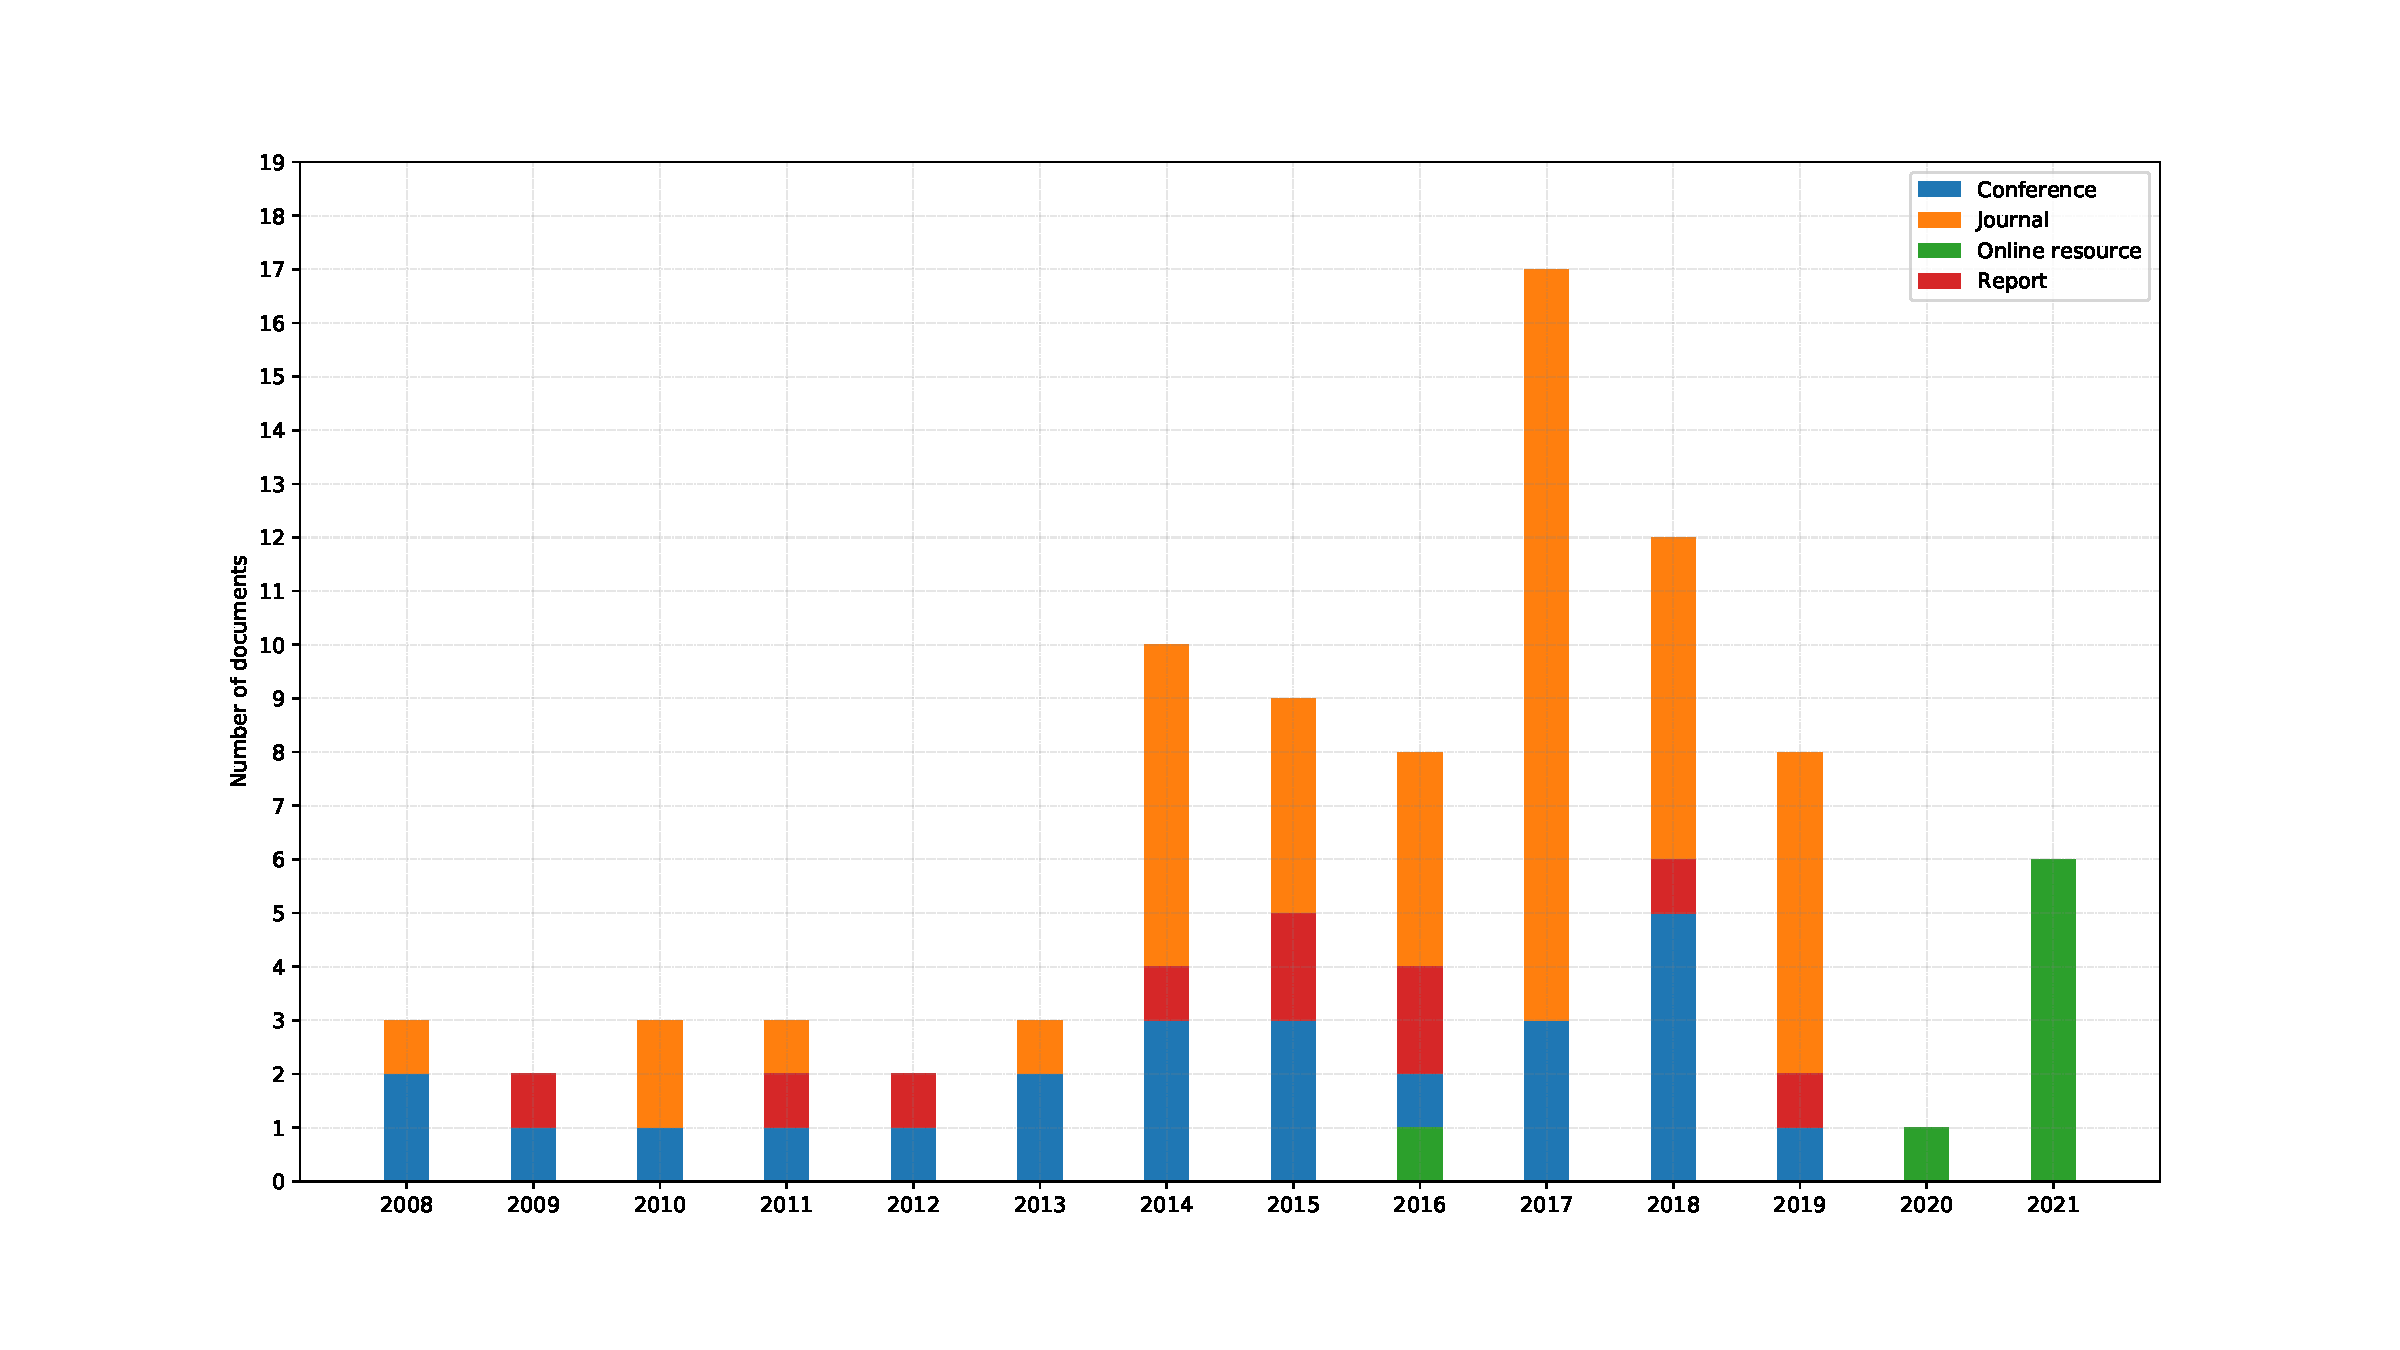
\includegraphics[width=15cm]{document_type.pdf}
    \caption{Number of documents as a function of the year and by type of document (publication venue)}
    \label{fig:type_of_article}
\end{center}
\end{figure}


\begin{table}[ht!]
\centering
\begin{tabular}[ht!]{p{0.04\textwidth}ccccc}
\hline
&Journal&Conference&Report&Online&\bf{Total}\\
\hline
\bf{IEEE}&27&24&-&-&\bf{51}\\
\bf{Elsevier}&14&-&-&-&\bf{14}\\
\bf{MDPI}&8&-&-&-&\bf{8}\\
\bf{USDOT}&-&-&4&5&\bf{9}\\
\bf{Springer}&7&-&-&-&\bf{7}\\
\bf{Other}&7&1&8&3&\bf{19}\\
\hline
\end{tabular}
\caption{Number of documents per publisher (\acrfull{IEEE}; \acrfull{MDPI}; \acrfull{USDOT}). }
\label{tab:publisher}
\end{table}

As the table~\ref{tab:publisher} shows, the main publisher for the documents is the Institute of Electrical and Electronics Engineers (IEEE) with 47~\% of all documents. % This is due to the additional research seen in the previous sections.
As discussed above, starting with the technical reports, in particular by \acrshort{ETSI}, which provided good initial classifications of the \acrshort{CT} applications, additional research for each specific application was done and often lead to papers published in IEEE journals and conference proceedings. One should also note the share of documents (13~\%), mainly scientific papers, published by Elsevier that provided crucial information for the construction of the taxonomy, in particular information from the journal \emph{Transportation Reasearch Part C: Emerging Technologies}

\subsubsection{Document Content}
%The strategy of this research, as mentioned in the previous sections, is to merge the telecommunications information and the transport information. To do this, two steps were taken to collect information from the papers. The first step focused on taxonomies / classifications of applications that allow us to obtain multiple information. With both a wide range of specific applications but also various elements related to telecommunications technologies. The step consisted of a more in-depth or complementary research on the missing information. This information concerns both the specific applications but also the different entities.

The document content was classified in the following categories: 
\begin{itemize}
\item Classification: documents dealing with transportation and/or telecommunication concepts providing a classification of these concepts, instead of a focus on a single entity;
\item Specific Classification: documents dealing providing a classification of transportation and/or telecommunication concepts, focusing on a specific sub-domain instead of attempting a comprehensive classification. An example is a document dealing only with road safety applications.  
\item Specific Application: documents dealing only with a specific \acrshort{CT} application, or a very small number.
\item Specific Technology: documents dealing with a single telecommunication technology, or a very small number. 
\end{itemize}


The resulting classification of the documents is presented in Fig~\ref{fig:information_article}. The documents providing ``general'' classifications and specific classications form the basis for the construction of the taxonomy, about 34~\% of all documents. They usually also provided a lot of information on the different attributes for the \acrshort{CT} applications and communication technologies. Documents on specific applications and technologies let us fill in missing information,
% The fact that specific searches are lower than other types of papers results in very complete information about classification papers, however specific searches have sometimes confirmed certain information of the classification,
for example the \acrshort{KPI}s of wireless telecommunication technologies like 5G.

\begin{figure}[ht!]
  \centering
  % \begin{subfigure}[b]{0.5\textwidth}
  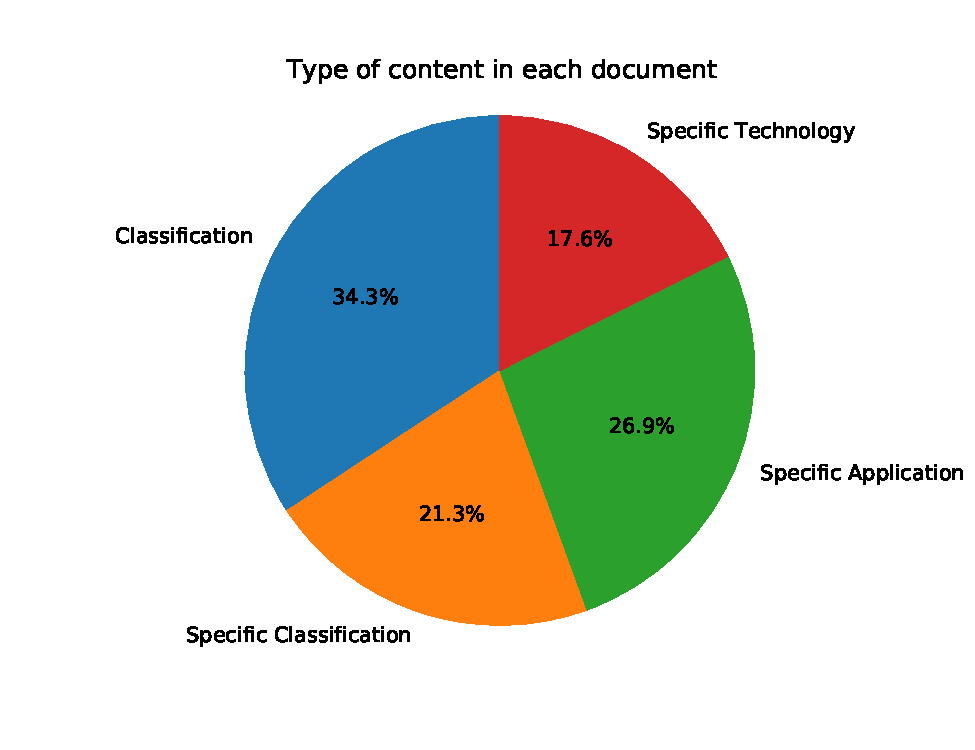
\includegraphics[width=0.33\textwidth]{pie_chart.pdf}
  % \caption{Type of content in each document}
  % \label{fig:pie_chart}
  % \end{subfigure}
\hfill
  % \begin{subfigure}[b]{1\textwidth}
  \includegraphics[width=0.66\textwidth]{information_article.pdf}
  %\caption{Number of documents mentioned each topic.}
  %\label{fig:witouth_ter}
  % \end{subfigure}
\caption{Distribution of the document content (on the left) and proportion of documents mentioning each topic (on the right) }?
    \label{fig:information_article}
\end{figure}



The topics discussed in each document were identified and are presented in Fig.~\ref{fig:information_article}. The most frequent topics are information on specific \acrshort{CT} applications and wireless technologies, which represent respectively 67.5 and 70~\% of the topics covered in the documents. At the other end, topics like the type of road users involved are rarely discussed in the documents (only in 2.78~\%). 
% However, other information which is not very present in the papers but which is very important, such as the types of users were identified in our research,0,7\% .
There are unfortunately fewer documents describing the requirements for each \acrshort{CT} application or the performance of each communicating technologies. These documents are still considered in our set of documents as they may be the only ones to cover a specific application or discuss a new communication technology. 
% Finally, it should be noted that in some papers, specific technologies and applications are discussed, without taking into account the requirement, this type of paper is still necessary for the construction of our taxonomy because it allows both to add additional information but also sometimes to identify technologies not present in the KPI studies . 

\subsection{Taxonomy}
\subsubsection{Definitions}

A taxonomy, originally used in biology, is ``the practice and science of classification of things or concepts'', and also refers to a ``specific classification scheme'' (Wikipedia) \cite{wikipedia_taxonomy_2021}
% More precisely, it is a science of classification that is widespread
It has become synonymous with classification and quite common in all scientific and technical fields. This makes it possible to group together concepts or objects. The goal of this paper is to classify \acrshort{CT} applications both in terms of abstract concepts like transportation application categories (e.g., safety) and of objects like communication technologies. 

\subsubsection{Taxonomy construction}

The taxonomy was build in three main steps. The first step started with the transportation field and the study of \acrshort{CT} applications. The area(s) or categorie(s) and other attributes of each application were identified and similar applications were grouped together. This resulted in a list of areas and attributes that were chosen based on the literature and our understanding of the applications. 
%More precisely that we group the applications according to transport criteria. This can be groupings in terms of "definition", for example two applications are close to transport safety applications. But we will also take into account other classification criteria such as types of users, type of roads, etc. 
The second step consisted in studying the \acrshort{CT} applications in the context of telecommunication technologies. The requirements and mode of communication (e.g.\ \acrshort{V2V} and/or \acrshort{V2I}) of each application to enable their proper implementation were researched. On the other side, the corresponding performance and attributes of current communication technologies were also documented. 
The last step was to match or map the two fields, in order to identify the possible communication technologies for each \acrshort{CT} application based on their respective performance and requirements. The results can be investigated in several ways, for example to study the requirements and suitable communicationt technologies by transportation categories. 
%the class to which it belongs and what technologies can be used for the proper implementation of these applications. But also by looking at other criteria such as the articulation of each transport class of representative KPIs.  This point is one of the innovative features that this paper brings to transport classifications. 

\subsubsection{Representation}
There is no one way to represent a taxonomy, especially this taxonomy as it connects two differents fields, and the attributes and their relationships are complex.
Multiple representations can be used, for example hierarchical representation like trees for 1 to $n$ associations, or graphical representations like Sankey diagrams for more general $m$ to $n$ associations. The choice depends on the goal of the representation and how it can be interpreted. 
%In our case, as we will see in the result part, we will take a large number of representations according to the chosen concepts. This can range from tables to Sankey for transportation categories. 

%This part is all the more important as it allows to have credible arguments on the chosen classification but also to make the classification visible to the reader. 

The most important representations are presented as tables and figures in this paper. The information about the documents, \acrshort{CT} applications and communication technologies gathered in this project is shared on a public GitHub repository~\url{https://github.com/HuguesBlache/taxonomy}, along with Jupyter notebooks containing the Python code to generate the figures presented in this paper. This repository contains other figures, as well as interactive visualizations (charts) using the plotly library that can be run on the binder platform \url{https://mybinder.org/}. Sharing the data and the code used to produce the results presented in this paper allows other researchers to build upon this work. 

% \paragraph{Visualisation}

% The graphics in this paper were built on a Jupyter-NoteBook using extensively the Plotly scientific graphics libraries. One of the advantages of these charts is that most of the charts and tables you create are interactive. 

% \paragraph{Interactive}

% To give a more dynamic reading to the reader, all the programs, which made it possible to directly construct the figures, were compiled in mybinder and depedantes of the database. For more explanations, a GitHub has been built in open access:  HuguesBlache/Taxonomy
 



\section{The Taxonomy}\label{sec:taxonomy}

The taxonomy based on the set of documents found in the literature is presented in three parts. The first consists in the taxonomy of \acrshort{CT} applications. The second part covers the communication technologies, both the requirements of the \acrshort{CT} applications and the characteristics of the technologies. The third and last part maps the technologies that can be used for each application. 

\subsection{\acrshort{CT} Applications}

%In this part, we will deal with the results we obtained during our data collection for the Transport part. To do this, it was necessary to distinguish between information disseminated for transport and telecommunications. For example, the specific application requirements (KPI) are intended for the telecommunications part because they are linked to the performance of wireless technologies. On the other hand, the type of road that the application can deploy will be a transport criterion.

This section will cover the various attributes used to differentiate the \acrshort{CT} applications. There are many ways to categorize these applications, in particular with various degrees of detail: for example, how many different vehicle type warning applications or collision risk warning applications should there be? The attributes, in particular the \acrshort{KPI} requirements, are key, as the goal of the taxonomy is to identify possible communication technologies for each application. Similar applications with the same attributes can thus be grouped. 

%To differentiate transport applications, we have chosen several criteria. We asked ourselves how far we should go. For example, for \textit{"Overtaking vehicle warning"} applications, should we differentiate between right and left overtaking applications? If we wanted to do purely transport application taxonomies, we could have separated them. But as for these two applications the requirements (KPI) are identical for its correct functioning, we have decided to merge them into a single application: \textit{"Overtaking vehicle warning"}. Other examples, we wondered, what should we collect or distinguish between apps? For example for the applications \textit{"Across traffic turn collision risk warning"} and \textit{"Merging traffic turn collision risk warning"}, if the applications deal with \textit{"Traffic turn collision risk warning"}, we have considered that communications and messages transmitted during communication are fundamentally different.

Following the information collected in the various documents, all applications were grouped into 61 distinct applications for this taxonomy. All the applications with their acronyms and their definitions are presented in~\ref{appendix:app}. 
The various attributes used to describe the applications are presented in the rest of the section. All attributes are non-exclusive, i.e.\ an application can take several possible values of each attribute. 
%For each specific application, we can issue a definition that is as exhaustive as possible and assign specific attributes to it. These attributes, we can list them in terms of different classes. For example the transport category (safety application or efficiency application) but also other classes such as the roads type or the users types that we will see in the rest of this article.


\subsubsection{Categories}
The first attribute deals with the nature of each application, i.e. the type of use the application will have for transportation or the type of impact the application will have on transportation. Categories include safety, efficiency and the environment. The categories were treated as non-exclusive, with each application possibly attached to several categories: for example, an intersection management application can improve both safety and efficiency. The categories result in a classification of the applications, which can then be analyzed at that level. The categories are also broadly related to their priority, for example safety has a higher priority than other applications in most situations. 

%One of the most relevant elements that we encountered in our reflections and in the articles read was the grouping of the different specific applications in terms of category or even sub-category. We could see that these elements are essential to identify the nature of a specific application, but also to see similarities in terms of requirement for each group of applications. So we will see what type of category we could have:

% {\bf BRUNI: jusqu'ici on a parlé de classes et subclasses. par contre, ci-dessous on parle de catégories. Donc, ça a l'air comme de quelque chose désagregé avec ce qu'on dit au-dessus} 

%{\bf Category}

% In the articles we have read, especially in the articles dealing with the taxonomy of transport applications, that specific applications can be grouped in terms of transport category. These categories make it possible to quickly know the importance and priority of specific applications, for example depending on traffic situations, a safety application will have priority over an infotainment application. But these categories also make it possible to verify the needs, of which we are in the telecommunications part.

Categories were added iteratively as applications were identified, adding new ones as applications did not fit existing ones. 15 categories were identified at the end of the proecess: 

\begin{enumerate}
\item[$A1$] the \textbf{safety} category deals with applications that aim to improve safety, i.e. by drecreasing the risk of a crash~\cite{hamida_security_2015};
  %groups together all the applications which aim to help all transport players (driver, vehicles, infrastructure, etc.) by transferring information on all situations, in particular on dangerous situations such as accidents \cite{hamida_security_2015}
\item[$A2$] the \textbf{efficiency} category deals with applications that aim to improve traffic by avoiding lost time and stops through data collection and sharing, and optimal vehicle control~\cite{hamida_security_2015};
  %collecting the different positions and statuses of transport players. 
\item[$A3$] the \textbf{entertainment} category covers the applications that provide users with access to the internet and media for their entertainment~\cite{hamida_security_2015};
  % gathers the applications which make it possible to transmit an access to multiple data to the user, in particular with the access to Internet. Which allows users to have fun or work 
\item[$A4$] the \textbf{confort} category includes the applications that aim to increase the comfort of road users~\cite{hamida_security_2015};
\item[$A5$] the \textbf{security} category includes the applications that aim to make road users more secure, e.g.\ to avoid the theft of a vehicle or to intervene in case of an emergency (other than for a crash); 
\item[$A6$] the \textbf{parking} category deals with applications that aim to help a driver park one's vehicle; 
\item[$A7$] the \textbf{environnement} category deals with application that aim to decrease the environmental impacts of transportation~\cite{chang_estimated_2015};
\item[$A8$] the \textbf{data collection} category relates to applications that collect data about any of the component of the transportation systems, vehicles, the infrastructure or users;   
\item[$A9$] the \textbf{freight} category deals with applications for freight (the movement of goods);
\item[$A10$] the \textbf{energy} category covers applications that aim to manage energy consumption, without an explicit goal to decrease the potential environmental impacts;
\item[$A11$] the \textbf{vehicle maintenance} category covers applications that aim to help with vehicle maintenance;
\item[$A12$] the \textbf{economic} category deals with applications that support the purchase of transportation services, economic activity and other economic aspects of transportation;
  % cost of transportation or to support the economy through the movement of people and goods;
\item[$A13$] the \textbf{access} category deals with applications that manage the access of users or vehicles to specific roads or zones; 
\item[$A14$] the \textbf{shared transport} category includes applications to share vehicles or manage fleets of vehicles;
\item[$A15$] the \textbf{traveler information} category deals with applications that provide useful information to users about their trips.
\end{enumerate}

Since an application can belong to several categories, the relationship between applications and categories is many-to-many. For example, a \emph{Speed Limit} application relates to safety, efficiency, the environment and energy. Such a relationship can be naturally represented as a bypartite graph or a Sankey diagram, as done in Figure~\ref{fig:app-category}.

It should be noted that some documents used sub-categories, for example of the different types of safety applications, but that most generally put each application in only one category. The sub-categories were not retained for this taxonomy for two reasons. The main was that sub-categories were not relevant for the telecommunication technologies: applications in the same sub-category generally had the same \acrshort{KPI} requirements. Second, sub-categories appeared often arbitrary and did not exist for all categories. 

%{\bf Sub-Catgory}

%The presence of transport subcategories was mentioned in the various articles studied and was the subject of reflection for the construction of the taxonomy. These subcategories correspond to categories within the categories formulated above. For example, a safety application can be classified in a subcategory of the type: Collossion application, road hazard warning application / road sign notification ect . 
%This classification in terms of transport has a certain logic because it allows to separate and atomize the applications for more specific research. But since the taxonomy relates to the requirements of specific applications, it was noted that the subcategories do not differentiate applications in terms of telecommunications. For example, for safety applications, the message sizes are similar, but totally different for infotainment applications. 
%It is with this type of reflection that on the one hand the classifications of the sub-categories have not been taken into account, but also to facilitate the understanding of the taxonomy. 

\begin{figure}[ht!]
  \begin{center}
    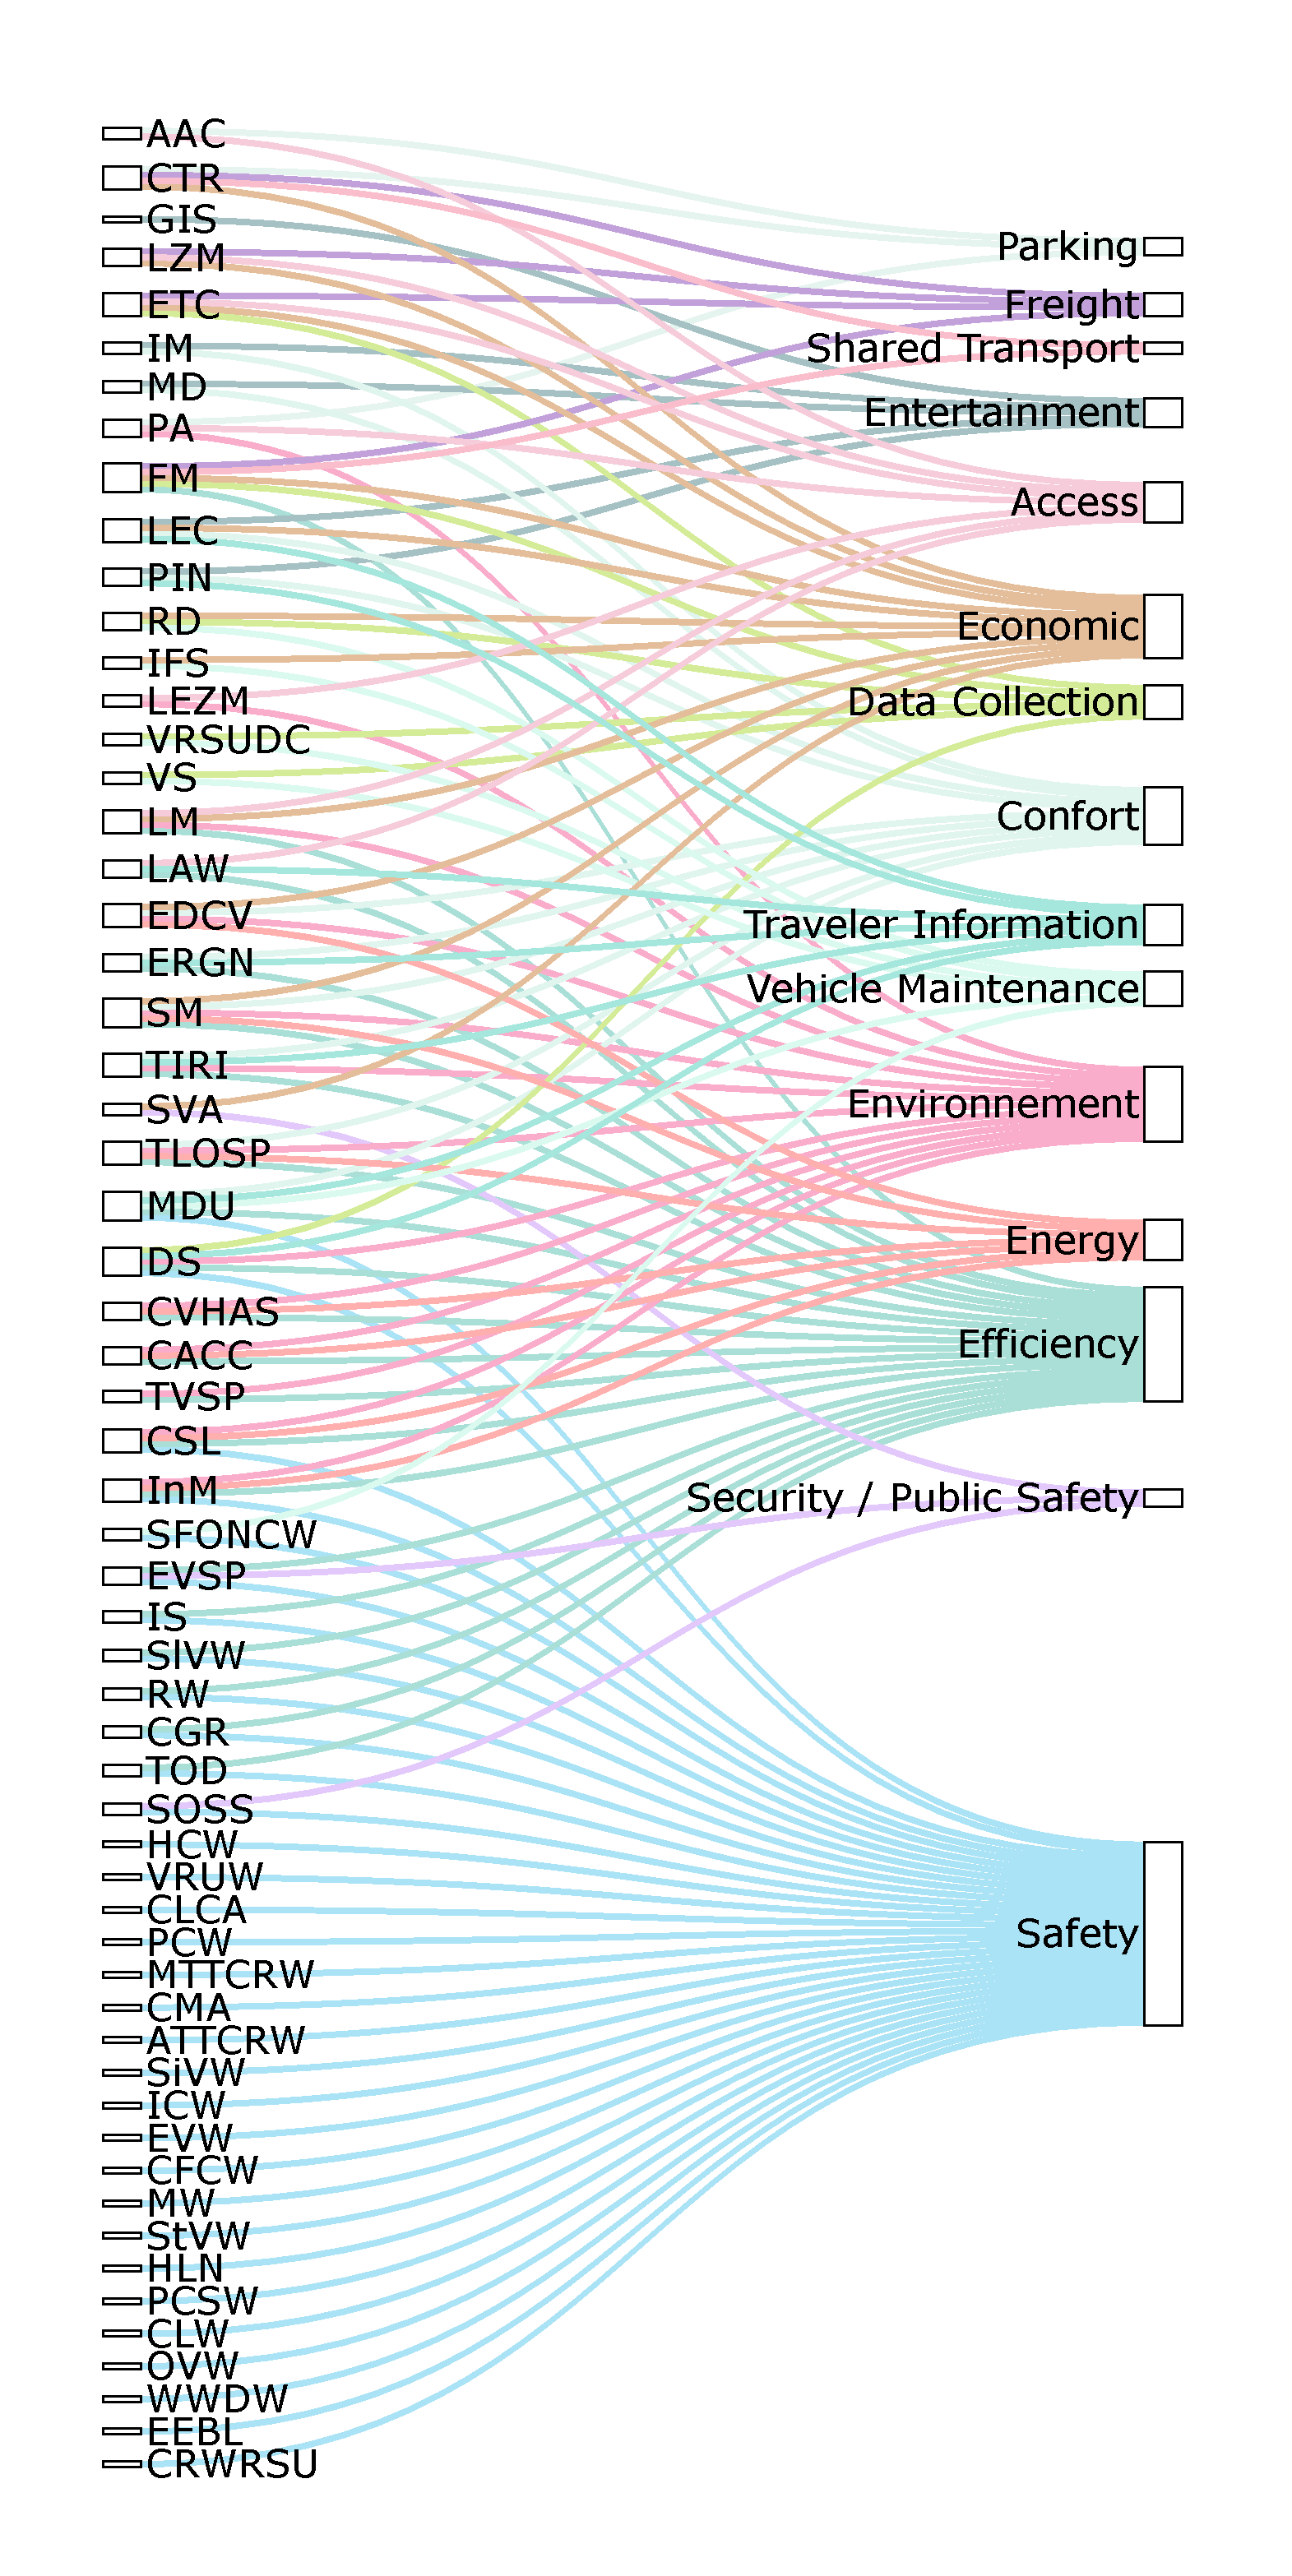
\includegraphics[width=0.7\textwidth]{category_sankey.pdf}
    \caption{Illustration of the application categories (see section~\ref{appendix:app} for the acronyms).}
    \label{fig:app-category}
  \end{center}
\end{figure}
%\FloatBarrier

\subsubsection{User Types}
The next attribute is the type of road user that may be involved in the use of the application or receive information or a warning from it.
% This attribute is obviously related to the mode of communication, e.g.\ vehicle to vehicle (V2V), vehicle to infrastructure (V2I) and vehicle to pedestrian (V2P).
Deciding which type of road user is involved is not always easy, as the main user of most applications is a driver of a passenger car or a commercial vehicle. The possible user types are listed below:

% Another useful classification is to focus on the type of user involved in each specific application. This type of classification has many advantages, it makes it possible to see which user is involved in the transport on the one hand and on the other hand it makes it possible to identify whattype of communication mode may be involved. For example if a specific application affects a vehicle and a pedestrian, we can expect the application to be V2P, even if the application implies that a vehicle is a transport provider, we can expect an application of type V2I. 

\begin{enumerate}
\item[$U1$] \textbf{Driver}: this category includes motorcyclists, commercial vehicle and public transit drivers; 
  % This category corresponds to people who drive or not a motorized vehicle on the road. These vehicles can range from cars to simple bikes
\item[$U2$] \textbf{Passenger};
  % Corresponds to people who move passively, that is to say who are not the driver of the vehicle transporting it.
\item[$U3$] \textbf{Pedestrian};
  % Corresponds to the person who does not use material means to move around
\item[$U4$] \textbf{Cyclist};
\item[$U5$] \textbf{Motorcyclist};
\item[$U6$] \textbf{Public Transit Driver};
\item[$U7$] \textbf{Commercial Vehicle Driver}.
  % Public or private entity that offers transport services, such as public transport for example. Actors indirectly linked to the mobility of the driver, who offers offers adapted to the user who wants or who travels and influences his movements. These could be, for example, parking lot operators
\end{enumerate}

Motorcyclists, commercial vehicle and public transport drivers are selected when an application specifically targets them. All applications with the driver attribute are relevant for all drivers, regardless of the specific vehicle. 
% The relationship between the applications and road user types is shown in a Sankey diagrame in Figure~\ref{fig:user_by_app}.
The number of applications per road user types is shown in Figure~\ref{fig:nb-app-attribut}. 

\begin{figure}[ht!]
  \begin{center}
    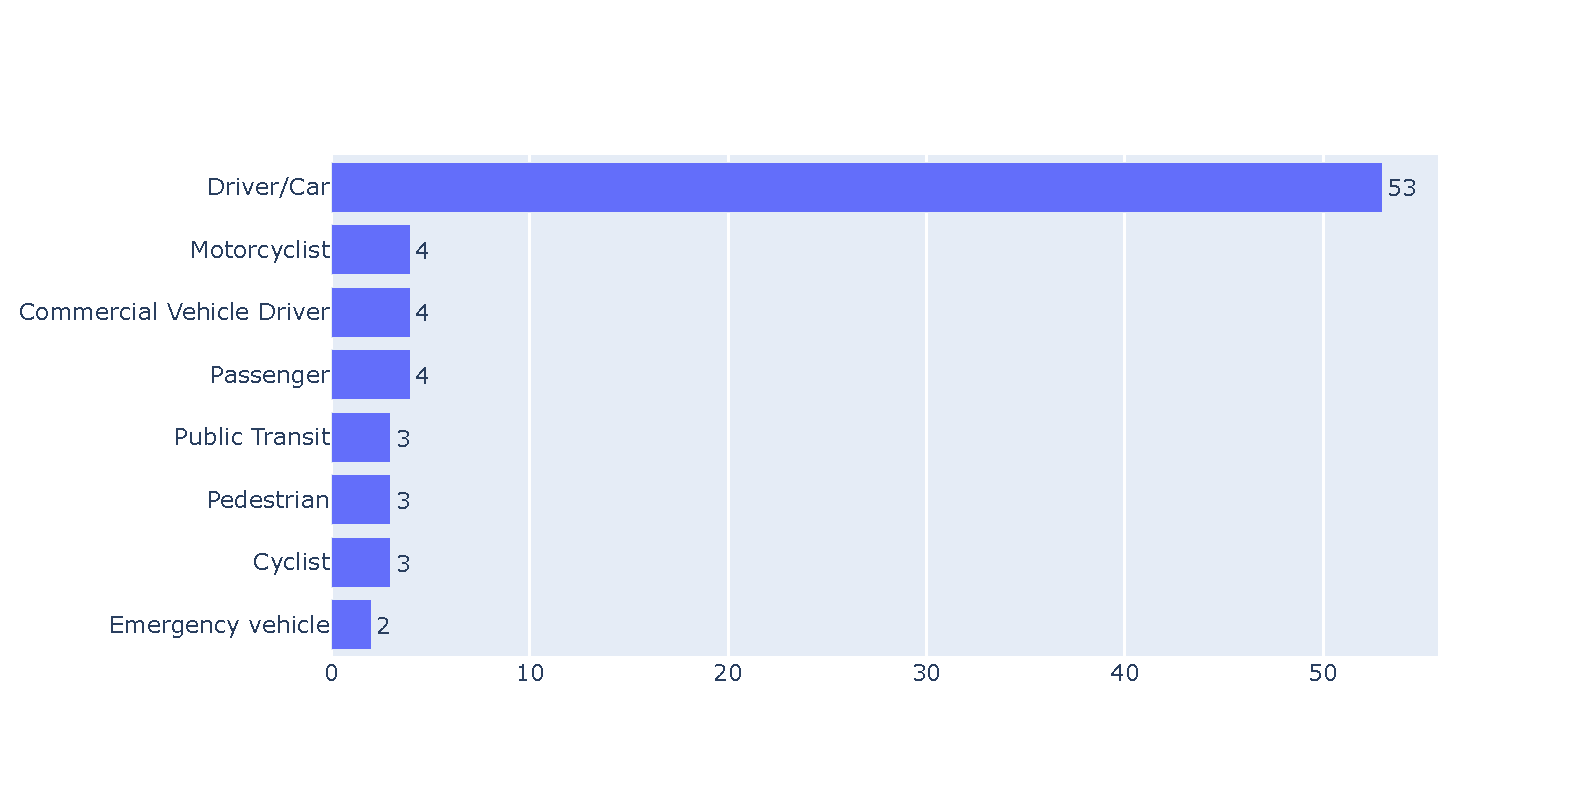
\includegraphics[width=0.5\textwidth]{diagramme_bar_attribut/user_types.pdf}\\
    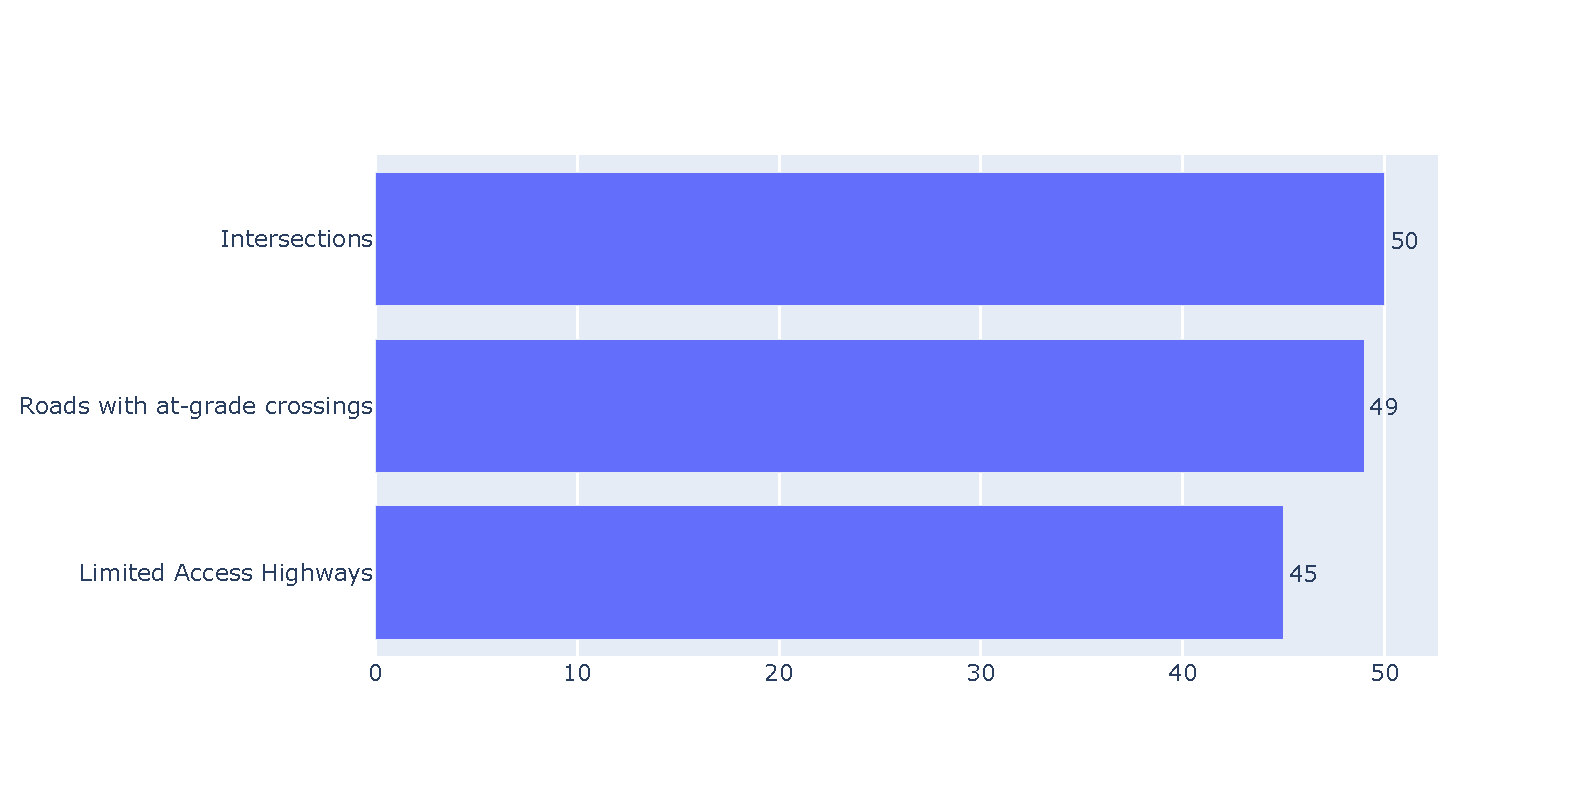
\includegraphics[width=0.495\textwidth]{diagramme_bar_attribut/road_types.pdf}
    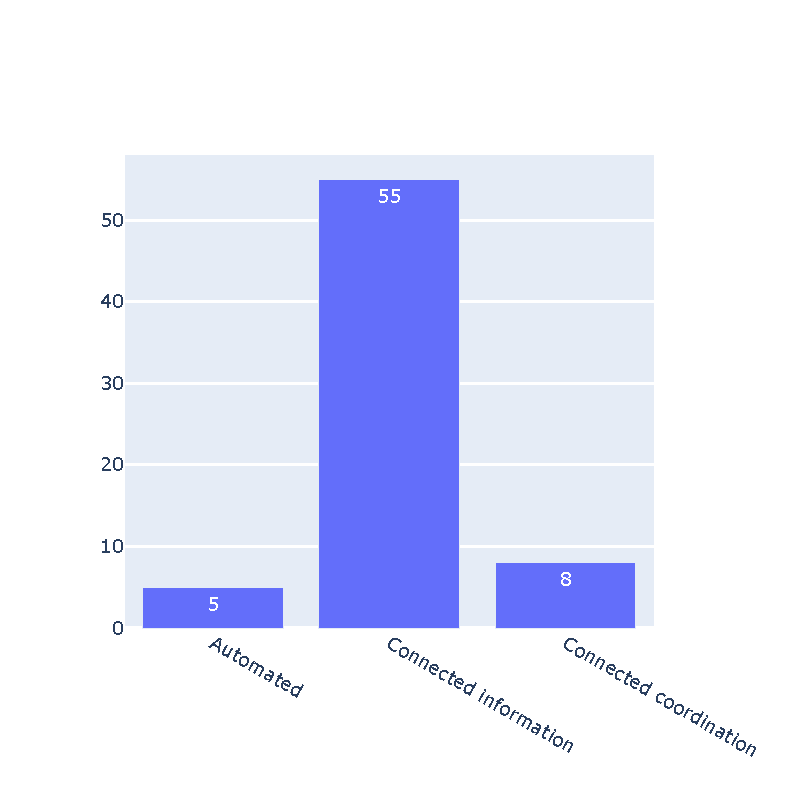
\includegraphics[width=0.495\textwidth]{diagramme_bar_attribut/mechanisms.pdf}
    \caption{Distribution of the number of applications according to road user types (top), road types (bottom left) and application mechanisms (bottom right).}
    \label{fig:nb-app-attribut}
  \end{center}
\end{figure}


\subsubsection{Road Type}
% Regarding transport, we can classify the different applications according to different criteria, we have seen that it is possible to do this in terms of transport categories and in terms of user type. Another class which is interesting and makes it possible to distinguish the type of road taken into account for the good implementation of specific transport applications.
Another important attribute relates to the parts of the networks where each application exclusively or typically operates. There are qualitative differences in the type of traffic on road segments and at intersections, and whether the intersections on a segment are at grade or not. This is related to the first two functions of roads, access and transit, which are inversely correlated: the more access to adjacent properties a road provides, the less important the transit function of the road, implying lower speeds. 
The following types of roads or parts of the network are considered:

%This type of classification has several effects, first of all we can assign road types to each application, for example applications of the type "Traffic light optimal speed advisory" cannot in theory be taken in roads Limits Access Highways on the other hand in the Intersections it can be integrated. The other effects come from the deployment of technologies that we will see in the rest of the article. Indeed, depending on the type of road, the type of infrastructure may be different and therefore the type of wireless technologies may be different. 


\begin{enumerate}
\item[$R1$] {\bf Limited access highways} are roads without any access to adjacent properties and no at-grade intersections. On such roads, one can move at high speeds without having to stop at intersections: traffic can be continuous (uninterrupted) as the only hindrance is other road users;% High speed road with few or no intersections 
\item[$R2$] On {\bf roads with at-grade intersections}, vehicles may have to stop at intersections, e.g.\ controlled by traffic control devices such as stop signs and traffic lights, and also for other modes of transportation such as public transportation and walking: such traffic is called discontinuous;
  % provides more access
  % Moderate speed road with at grade corssings
\item[$R3$] {\bf Intersections} of roads or with infrastructure for other modes of transportation are the most complex part of a road network, involving issues of safety and efficiency that traffic and priority rules attempt to address. %Low speed road with intersections like traffic light
\end{enumerate}

As can be seen in Figure~\ref{fig:nb-app-attribut}, most applications apply to all these road types, but some are only relevant to one, e.g.\ to intersections in the case of traffic lights, or to roads with at-grade intersections in the cases where the application requires access to adjacent property, which is not possible on limited access highways. 


\subsubsection{Application Mechanisms}
The last attribute is the mechanism by which the application has the desired effect. Connectivity between vehicles, users and pieces of infrastructure let them exchange data and information, which can be used in different ways, most importantly to inform the driver for him to make decision and take action, or to let the vehicle in some cases take action in an automated way. The application mechanism is thus categorized as:

%A last classification in connection with the telecommunications part and which is for us a category which will take more and more place in future research of communication transport applications, is the classification of application mechanisms. This category concerns automation and the nature of the information transmitted between each type of user. To do this, we can distinguish two types of information (and decision) transmitted in the applications:

\begin{enumerate}
\item[$AM1$] {\bf Connected information}: such applications provide data and information obtained through communication with other vehicles, users and pieces of infrastructure to the driver who has the control of the vehicle: this implies that the driver can ignore the information of the \acrshort{CT} application;
  %This type of information takes into account the information transmitted by a vehicle or an infrastructure to other traffic users without any cooperation in decisions. This is the case, for example, with the \textit{"Pre-Crash sensing Warning"} application where information is transmitted on unavoidable accidents but the information will be taken without taking into account the condition of other road users.
\item[$AM2$] {\bf Connected coordination}: such applications not only exchange information between vehicles, users and infractructure, but also let the vehicles coordinate to find a solution that is better for all users than any solution that could have been found if each user decided separately;\\
  a good example is ``Co-operative adaptative cruise control'' where users can coordinate to select the optimal braking rate to avoid a crash and optimize other impacts such as energy consumption;
  % This type of information is a special case of connected information. In this case, we classify the applications where information and decision-making are done collectively in a coordinated manner between users. For example, in the case of platoon-type applications, vehicles will collectively make decisions to optimize their speed and other elements.
\item[$AM1$] {\bf Automated}: such applications use the data and information they receive to directly control at least one function of the a vehicle such as acceleration or braking. 
\end{enumerate}

This attribute is important for the efficiency of the applications, as coordinated or automated applications will be more effective than what the driver may do based on the provided information. It is also related to some communication \acrshort{KPI}s as coordination will require more data exchanges for the vehicles to make a decision collectively. It should be noted that applications that support infotainments services, \acrfull{GIS}, \acrfull{IM} and \acrfull{MD} do not correspond to any of the above categories. From the number of applications per mechanism types shown in Figure~\ref{fig:nb-app-attribut}, it is obvious that the vast majority of \acrshort{CT} applications only provide information to the driver. 

%As for the categories of transport, the choice of the representation of the road types was a sankey  Fig  \ref{fig:application_mecanisme}

\subsection{Telecommunication Technologies}
%After having seen all the useful classifications for the transport part for the different specific applications, we will focus on the telecommunications part. 
%To do this, focusing on the objective of the article, if possible, note the requirements of specific applications and assimilate to each specific application the wireless technologies that can be used.
%To do this, we will do two studies in this part of telecommunications, first we will focus on current wireless technologies that take into account their performance and secondly we will focus on the requirement of each specific application. 
The first step is to define the main \acrshort{KPI}s used to describe the \acrshort{CT} application requirements and the telecommunication technology capabilities. Second, the wireless telecommunication technologies that may be used in \acrshort{CT} applications are listed. They are often discussed in the literature under the topic of vehicular ad hoc networks (VANET). These technologies fall into three categories: short (below 100~m), medium (between 100~m and 1~km) and long range (above 1~km)~\cite{anwer_survey_2014,shree_novel_2016}. 
The characteristics of the different technologies are presented in each category. 
The last step is to present the modes of communications related to the components of the transportation networks involved in the various transportation applications. 
Figure~\ref{fig:wireless_techs} depicts the wireless technologies in terms of transmission range and data rate.

\begin{figure}[ht!]
  \begin{center}
    \includegraphics[width=0.5\textwidth]{../image/wireless_technologies.jpg}
    \caption{Communication technologies as a function of range and data rate. {\bf NS: refaire en pdf}}
    \label{fig:wireless_techs}
  \end{center}
\end{figure}

\subsubsection{Telecommunication and Application KPIs}

%In this part, we will now focus on the telecommunications aspect for specific applications, that is to say the sufficient criteria for the proper functioning of the latter. To do this, like the technologies, we will separate two studies, first we will look at the KPIs of the applications and secondly we will analyze the modes of communication deployed for these specific transport applications. 

\acrshort{KPI}s may be qualitative or quantative. There are many \acrshort{KPI}s used in the literature and not all are relevant for this taxonomy. In particular, all the \acrshort{KPI}s that allow to link the requirements of \acrshort{CT} applications to the performance of communication technologies were kept. They are defined in the following list in terms of requirements for the functioning of the applications:
%There is a lot of information in the articles about the different specific applications, so it is important to choose the KPIs that are useful for our studies. We therefore decided to take the 

\begin{enumerate}
\item the {\bf latency} is the maximum duration allowed to carry out the communication~\cite{etsi_etsi_tr_102_638_intelligent_2009}; %  for the proper functioning of the application
\item the {\bf range} is the minimum distance at which information should be transmitted between the users, vehicles and units involved;
\item the {\bf message frequency} is the number of messages transmitted by the application per unit of time;
\item the {\bf message size} is the size of the message transmitted during the communication; {\bf NS: size up or just size?}
\item the {\bf data rate} is the minimum rate of data transmitted during the communication of the application; %It is often expressed in bits/s
\item the {\bf priority} represents the relative importance of messages across different applications. For example, security messages take priority over infotainment messages. There are three levels: high, medium and low; 
\item the {\bf message type} is the nature of the message transmitted, for example whether it is periodic or not. 
\end{enumerate}

When not available, the data rate is derived as the product of the message size mutiplied by the message frequency. The communication technologies are described with a few attributes, namely the relevant standard, frequency and bandwidths, and the following extra \acrshort{KPI}s:

\begin{enumerate}
\item signal interference;
\item accessibility;
\item security.
\end{enumerate}
% Standard & Data Rate & Range & Latency & Signal Interference  & Frequency & Bandwidths & Accessibility & Security

{\bf NS: definir ces KPIs\\
Brunilde, a relire les definitions (des KPIs ci-dessus et des technologies ci-dessous)}

It should be noted that the deployment of some technologies, namely the technologies forming cellular networks like 5G and LTE, is expected to be dense to cover most transportation facilities in such a way that the application range criterion will be met, independently of the communication technology intrinsic range (if it was sparsely deployed). 


%For an easier to understand representation of this article, a grouping of KPIs by category has been favored, as shown in the figure at parallel coordinates.


\subsubsection{Descriptions and Categories of Communication Technologies}
%In this part, we will list the different wireless technologies used in our study to build the taxonomy. To do this, we tried to take all the technologies that use the different modes of communication included in our taxonomy (V2V, V2I, V2P).
%In the literature, these technologies are often linked to the implementation of the ad hoc network of vehicles (VANET), which seemed relevant to our study. 
%Thus, after compilation of the data, we were able to take charge of categories of technologies according to their transmission range:

\paragraph{Short Range Communication Technologies}\ \\
Short range communication technologies, sometimes referred to as short-region wireless technologies~\cite{yu_technology_2018}, refer to technologies that communicate in a small region of the order of a maximum of 100~m. These types of technologies are more suitable for indoor applications as well as outdoor applications that require small distances between the equipments. Their \acrshort{KPI}s are presented in Table~\ref{tab:short-range-com}.
% and a minimum level of the order of a millimeter.

\begin{table}[ht!]
  \centering
  \caption{Short Range Communication Technology \acrshort{KPI}s}
  \label{tab:short-range-com}
  \begin{tabular}{p{1,4cm} p{1cm} p{1cm} p{1cm} p{1cm} p{1.5cm} p{1.2cm} p{1.3cm} p{1.4cm} p{1.4cm}}
    \hline
    Technology & Standard & Data Rate & Range & Latency & Signal Interference  & Frequency & Bandwidths & Accessibility & Security\\
    \hline
    UWB &  IEEE 802.15.3  & 480 Mb/s	&   10 m - 75 m	 &  0.1 ms  & Low & 3.1-10.6 GHz	 &500 MHz - 7.5 GHz	 & Contention based	& High\\
   
    Bluetooth  & IEEE 802.15.1	& 1-24 Mb/s	&  10 m&	100 ms  & High &  2.4 GHz	& 1 MHz& 	Schedule Based	& Low\\
	
    BLE  & IEEE 802.15.1	& 1 Mb/S	&  50 m& 6 ms & High&	2.4 GH &	2 MHz 	&Schedule Based&	Low\\

    ZigBee& IEEE 802.15.4	&20-250 Kb/s&	 100 m	&30 ms  &High	&868 MHz, 902–968 MHz and 2,4GHz	&2 MHz & Schedule Based	&High\\
    \hline
  \end{tabular}
\end{table}

\textbf{\acrfull{UWB}} is a technology belonging to the IEEE 802.15.3 standard which operates on a frequency band between 3.1 and 10.6~GHz and for a bandwidth between 500~MHz and 7.5~GHz~\cite{anwer_survey_2014,ahangar_survey_2021}. Being short range, this technology can send data up to 10~m for its best performance and up to 75~m with a minimum latency of 0.1~ms~\cite{ahangar_survey_2021}. Its highest data rate corresponds to 480~Mb/s~\cite{wang_networking_2019}. The advantage of UWB over most other short range technologies is that it experiences little interference during communication and is therefore ideal for dense areas and meetings in crowded places~\cite{ahangar_survey_2021}. 

\textbf{Bluetooth} technologies belong to the IEEE 802.15.1 standard which operates on a frequency band of 2.4~GHz and for a bandwidth of 1~MHz~\cite{anwer_survey_2014,ahangar_survey_2021}. Like UWB technologies, its range is around 10~m but with a low data rate of only around 1 to 24~Mb/s with a latency of 100~ms~\cite{ahangar_survey_2021}. While the advantage of Bluetooth is that it is present in our environment and is relatively inexpensive to deploy, it only connects two entities at a time and has very strong interference, which prevents from functioning well in very busy environments~\cite{wang_networking_2019,bluetooth_bluetooth_2021,akpakwu_survey_2018}. 

\textbf{\acrfull{BLE}} is a version of Bluetooth that consumes less energy while keeping the same performances remain except for the range up to 50~m with lower latency (6~ms). The advantage of course is that this technology consumes less energy but it is not compatible with the other Bluetooth standard that is very common in our environment~\cite{ahangar_survey_2021}. 

The \textbf{ZigBee} technology follows the IEEE 802.15.4 standard that uses different frequency bands like 868~MHz, 908-968Mhz~and 24~Ghz, for a bandwidth of 2~MHz~\cite{ahangar_survey_2021}. The advantages of this technology are the range of 100~m and the latency of 30~ms. However, the data rate is only 250~Kbps, making it a convenient technology for applications requiring small message sizes, regardless of the fact that this technology is susceptible to interference~\cite{anwer_survey_2014,ahangar_survey_2021,shree_novel_2016,selvarajah_zigbee_2008}. 

%\textbf{InfraRed}


\paragraph{Medium Range Communication Technologies}\ \\

\begin{table}[ht!]
  \centering
  \caption{Medium Range Communication Technologies \acrshort{KPI}s}
  \label{tab:medium-range-com}
  \begin{tabular}{p{1,4cm} p{1cm} p{1cm} p{1cm} p{1cm} p{1.5cm} p{1.2cm} p{1.3cm} p{1.4cm} p{1.4cm}}
    \hline
    Technology & Standard & Data Rate & Range  & Latency & Signal Interference  & Frequency &  Bandwidth & Accessibility & Security\\
    \hline
    Wi-Fi &  IEEE 802.11n  &  54 Mb/s	&   240 m &  50 ms  & High & 2.4-5 GHZ	 & 20 MHz	 & Contention based&	Low\\
    
    DSRC / Wave  & IEEE 802.11p	& 27 Mb/s	& 1 km&	100 ms  & Low &  5.9 GHz	& 10 MHz& 	Contention based &	High\\
    \hline	
  \end{tabular}
\end{table}

Communication technologies are most often classified in short and long range technologies. In our case, we decided to add a third category: medium range communication technologies with a range between 100~m and 1~km. Their \acrshort{KPI}s are presented in Table~\ref{tab:medium-range-com}.%Here are the technologies that we took in our study:

\textbf{\acrfull{Wi-Fi}} technologies follow the IEEE 802.11 standard. Its transmission range (250~m) sometimes puts it in the category of short range technologies~\cite{araniti_lte_2013,anwer_survey_2014}. This technology uses two frequency bands, 2.4~GHz and 5.2~GHz, with a channel bandwidth between 1~and 40~Mhz~\cite{papadimitratos_vehicular_2009}, has a low latency of 50~ms and a maximum throughput of 54~Mb/s~\cite{ahangar_survey_2021}. However, due to high interference with its communication environment, Wi-Fi seems difficult to be deployed for high density applications~\cite{chen_lte-v_2016}.

The \textbf{\acrfull{DSRC}} is based on IEEE 802.11p and is used both for \acrshort{V2V} and \acrshort{V2I} communications~\cite{ahangar_survey_2021}. This technology uses the 5.9~GHz frequency band with a 10~MHz bandwidth~\cite{ghosal_security_2020}. 
Its maximum range of 1~km with a data rate of 27Mb/s puts it in the medium range category~\cite{anwer_survey_2014}. It has a latency of 100~ms~\cite{ahangar_survey_2021}. Its advantages are its medium range, low latency and low interference, ideal for security applications. However, this type of technology is limited in the event of heavy congestion~\cite{cailean_survey_2014}. Wireless access in vehicular environments (WAVE) is considered along \acrshort{DSRC} because these technologies are almost identical, except for the physical layer~\cite{ghosal_security_2020}.

\paragraph{Long Range Communication Technologies}\ \\

\begin{table}[ht!]
  \centering
  \caption{Long Range Communication Technologies \acrshort{KPI}s}
  \label{tab:long-range-com}
  \begin{tabular}{p{1,4cm} p{1cm} p{1cm} p{1cm} p{1cm} p{1.5cm} p{1.2cm} p{1.3cm} p{1.4cm} p{1.4cm}}
    \hline
    Technology & Standard & Data Rate & Range  & Latency & Signal Interference  & Frequency & Bandwidth(s) & Accessibility & Security\\
    \hline
    Wi-Max &  IEEE 802.16m &100 Mb/s	& 15 km&  10 ms  & High & 2.5, 3.5, 5.8 GHz	 & 5, 10, 20MHz & Schedule Based&	High\\
    
    LTE-4G & 3GPP &1 Gb/s	&  11 km &  50 ms  & Low & 2-5 GHz	 &  5, 10, 15, 20 MHz	 &Contention based&	High\\
  
    5G - Low-band & 3GPP &250 Mb/s	&  15 km &  30 ms  & Low & < 1GHz	 &  800-1900 MHz	 &Contention based&	High\\
  
    5G - Mid-band & 3GPP &900 Mb/s	&  1 km &  10-20 ms  & Low & 60 GHz	 &  100 MHz	 &Contention based&	High\\

    5G - mmWave & 3GPP &20 Gb/s	&  100 m &  1 ms  & Low & > 24 GHz	 &  400 MHz	 &Contention based&	High\\

    NBIoT & 3GPP &200 Kb/s	&  10 Km &  50 ms  & Low &  2.4 GHz	 &  200 KHz	 &Contention based&	High\\

    MBWA & IEEE 802.20 &4.5 Mb/s	&  15 km &10ms & High & 3.5 GHZ 	 & 5, 10, 20 MHz  	 &Schedule Based&	High\\

    MicroWave & IEEE 802.15.4 &16 Gb/s	&  10 km &   & High & 	 &  	 &Contention based&	Low\\

    LoRa  &801.15.4g&50 Kb/s	&  5-15 km & 400 ms  & Low & 865 - 923 MHz	 & 125, 250, 500 Khz 	 & Contention based&High	\\

    SigFox  &3D-UNB &100 b/s - 600 b/s	&  10-50 km & 1s  & Low & 25 MHz - 1 GHz	 &  192KHz &Contention based&High	\\
   
    DASH7  &D7A &167 kb/s&  1 km &   &  & 433, 868/915 MHz	 &  25 kHz or 200 kHz	 &Schedule Based& High	\\

    Ingenu-RPMA  & IEEE 802.15.4k&624 kb/s&  45km &   &  & 2.4 GHz	 & 1 MHz 	 &&High	\\
    \hline
  \end{tabular}
\end{table}

Compared with the other communication technologies, the long range category contains technologies with a range greater than 1~km. Their \acrshort{KPI}s are presented in Table~\ref{tab:long-range-com}.

The \textbf{\acrfull{WiMax}} technology complies with the IEEE 802.16m standard and uses the 2.5~GHz frequency band. This long range technology can communicate up to 15~km~\cite{selvarani_comparative_2014} and transmit at a speed of 100~Mb/s~\cite{anwer_survey_2014} in the case of mobile transmission~\cite{selvarani_comparative_2014} with a latency of 10~ms~\cite{msadaa_comparative_2010}. The advantage of this technology is that it has a very large transmission range.

{\bf Hugues: Comme pour la 5G, verifier les valeurs des technologies}

The \textbf{\acrfull{LTE}} and \textbf{\acrfull{LTE-A}} technologies developed by 3GPP and marketed under the names 4G use a frequency band of 2~GHz~\cite{seo_lte_2016} and a bandwith that can go up to 100~MhZ~\cite{araniti_lte_2013}. %By separating 5G, the deployment capacity
The range can reach 11~km~\cite{shah_5g_2018} with a transmission of 1~Gb/s~\cite{araniti_lte_2013} and a low latency of 10~ms, which make this technology appropriate for all applications. 
%For simplicity and to avoid taking the less obsolete technologies, LTE-A includes LTE

The \textbf{5G} technology follows the 3GPP standard and is the latest version of mobile technologies about to be deployed in many cities. The latter is eagerly awaited for its performance and is expected to speed up the implementation of ITS applications~\cite{foubert_long-range_2020}. Unlike 4G, 5G could be deployed in three frequency bands: a low-frequency band (less than 2~GHz), a mid-frequency band (between 3~GHz and 6~GHz, often called sub-6~GHz band) and a high-frequency band (above 24~GHz, often called millimeter wave (mmWave))~\cite{foubert_long-range_2020}. 5G is intended to provide high data rate reaching 20~Gb/s~\cite{hussain_integration_2019}.
In addition, with this improved performance, a latency of less than 1~ms is expected~\cite{hussain_integration_2019} and a range between a few hundred meters and more than 10~km~\cite{foubert_long-range_2020}. This promising technology could address several shortcomings of current technologies, especially for security applications that use \acrshort{DSRC}~\cite{shah_5g_2018}. 

\textbf{\acrfull{NBIoT}} is a \acrfull{LPWAN} technology proposed by 3GPP for low cost, low battery life and \acrfull{C-IoT} applications~\cite{qadir_low_2018,routray_narrowband_2021}.

The \textbf{\acrfull{MBWA}} technologies follow the IEEE 802.20 standard, use the 3.5~GHz frequency band, and exchange at a data rate of 4.5~Mb/s in a communication area of 15~km \cite{anwer_survey_2014}.

% \textbf{MicroWave}

\textbf{\acrfull{LoRa}} uses different frequency bands depending on the continent, e.g.\ for the USA 915~MHz and 433~MHz~\cite{li_lora_2018}. Its deployment is different depending on the environment, going from 5~km in urban areas, up to 15~km in rural areas, with exchange rate at a speed of 50~kb/s~\cite{foubert_long-range_2020, queralta_comparative_2019} and a high latency (400~ms)~\cite{potsch_towards_2019}. This promising technology is a very low-cost solution, yet not feasible for latency sensitive applications given its high latency.

\textbf{SigFox} has a low data rate (100 to 600~bp/s) and a long range (10~km in urban areas and up to 50~km in rural areas)~\cite{potsch_towards_2019}. This technology uses a frequency band of 869 and 915~MHz and consumes very little energy~\cite{akpakwu_survey_2018}. Despite a large deployment, it would be difficult to use for \acrshort{CT} applications given the low data rate. 

The \textbf{DASH7} technology uses 433~MHz as the frequency band, at a low rate of 197~kb/s~\cite{akpakwu_survey_2018}. Unlike other long-range technologies, it has a range of 1~km in urban areas
% , which makes it a medium-range technology
, but is less efficient than \acrshort{DSRC}~\cite{foubert_long-range_2020}.

The \textbf{Ingenu-RPMA} technology is compliant with IEEE 802.15.4k standard~\cite{akpakwu_survey_2018} and uses the 2.4~GHz frequency band~\cite{foubert_long-range_2020}. 
Its range can reach 15~km in an urban environment, but it has a data rate of only 156~kb/s~\cite{foubert_long-range_2020} which makes it difficult to use for \acrshort{CT} applications. %to set up as part of a communication application}.

%We have just seen in this categorization the definitions of wireless technologies and their performance as a general telecommunication tool. But an important piece of information is in what type of communication mode can we use these technologies to be able to map them to each specific application requirements. 

\subsubsection{Modes of Communication}
% https://en.wikipedia.org/wiki/Vehicle-to-everything % vehicular communication systems
 
There are various types or modes of communication between the various components of the transportation system, generally centered on the vehicle communicating with a specific type or several types of road users~\cite{araniti_lte_2013,molina-masegosa_lte-v_2017,shladover_connected_2018,dar_wireless_2010,abboud_interworking_2016,chen_lte-v_2016}: 

%Connected cars can communicate in different modes, depending on the transmission and reception ways.. 
%Thus, we can take data to collect useful information on the deployment of technologies in communication modes, for example if a technology can be used in V2I communication 
%In general, the communication mode can be classified as follow:
% In our study, we decided to take into account only 3 types of communication: 

\begin{enumerate}
\item[$M1$] \acrfull{V2V} communications refers to vehicle-to-vehicle communications, without  the use of the telecommunications infrastructure;
  % In \acrfull{V2V} communications,  information are  exchanged directly between motor vehicles without the use of the telecommunications infrastructure. 
\item[$M2$] \acrfull{V2I} communications refer to vehicle-to-infrastructure communications, with various pieces of infrastructure like traffic controllers or sensors are equiped with communication modules that can connect to nearby vehicles;
% In \acrfull{V2I} communications , information are exchanged  between the vehicles and the telecommunications infrastructures. 
\item[$M3$] \acrfull{V2P} communications refer to vehicle-to-pedestrian communications, including pedestrians with mobility devices and cyclists. 
%In  \acrfull{V2P} communications , information are exchanged   between motorized vehicles and non-motorized vehicles such as pedestrians or bicycles. 
\item[$M4$] \acrfull{V2X} communications refer to two or more of the previous communications modes.
\end{enumerate}

\begin{figure}[ht!]
  \centering
  \begin{tikzpicture}[every text node part/.style={align=center}, thick, scale=1.5]
    \node[label={\small V2I}] (un) at(2.3,0){\includegraphics[width=.1\textwidth]{infra.png}};
    \node[label={\small V2V}]  (deux) at (0.8,-3){\includegraphics[width=.1\textwidth]{car.png}};
    \node (trois) at (2.3,-1.5){\includegraphics[width=.1\textwidth]{car.png}};
    \node[label={\small V2P}]  (quatre) at (3.8,-3){\includegraphics[width=.1\textwidth]{pedestrian.png}};
               
    \draw[<->,draw=green!70!red!50,fill=green!5,line width=0.2mm] (trois.north) -- (un.south);
    \draw[<->,draw=blue!90!black!70,fill=green!5,line width=0.2mm] (trois.south west) -- (deux.north east);
    \draw[<->,draw=red!70,fill=green!5,line width=0.2mm] (trois.south east) -- (quatre.north west);
  \end{tikzpicture}
  \caption{Communication Mode}
  \label{fig:com-mode}
\end{figure}

\acrshort{V2X} communications are not explicitly considered in our taxonomy: they can be inferred when a technology supports at least two of the other modes. 
%In our classification of communication modes, we did not consider V2X communication. For us, Vehicle-to-Any (V2X) communication is a communication that combines all previous communications. We therefore noted that if a technology was V2X, it could communicate with all the elements of the environment.
For example, 5G is a technology supporting the V2X communication mode, as it can be deployed for V2V, V2I and V2P applications. 
Some more specific modes of communication have not been taken into account, in particular because they are mostly redundant with the others or not relevant. For example, \acrfull{V2T}~\cite{vandung_nguyen_efficient_2016} and vehicle-to-bycicle/cyclist (V2C) are special cases of \acrshort{V2I} and \acrshort{V2P} communications respectively. 
% We have deliberately not taken into account certain modes of communication, whether it is poor appearance in our applications or redandance in other modes of communication. This is the case of \acrfull{V2T}\cite{vandung_nguyen_efficient_2016} which is, for us alone, a specific case of V2I, but also of Vehciule-to-bycicle, which is a special case of V2P.
% Following the example of the study of technologies, we research for each application which mode of communication is used.

% \begin{figure}[ht!]
%   \begin{center}
%     \includegraphics[width=16cm]{tech.png}
%     \caption{Modes of communication supported by each technology.}
%     \label{fig:mode-com-tech}
%   \end{center}
% \end{figure}
% \begin{figure}[ht!]
%   \begin{center}
%     \includegraphics[width=0.8\textwidth]{communication.png}
%     \caption{Modes of communication supported required by each application.}
%     \label{fig:mode-com-app}
% \end{center}
% \end{figure}

\begin{figure}[ht!]
  \begin{center}
    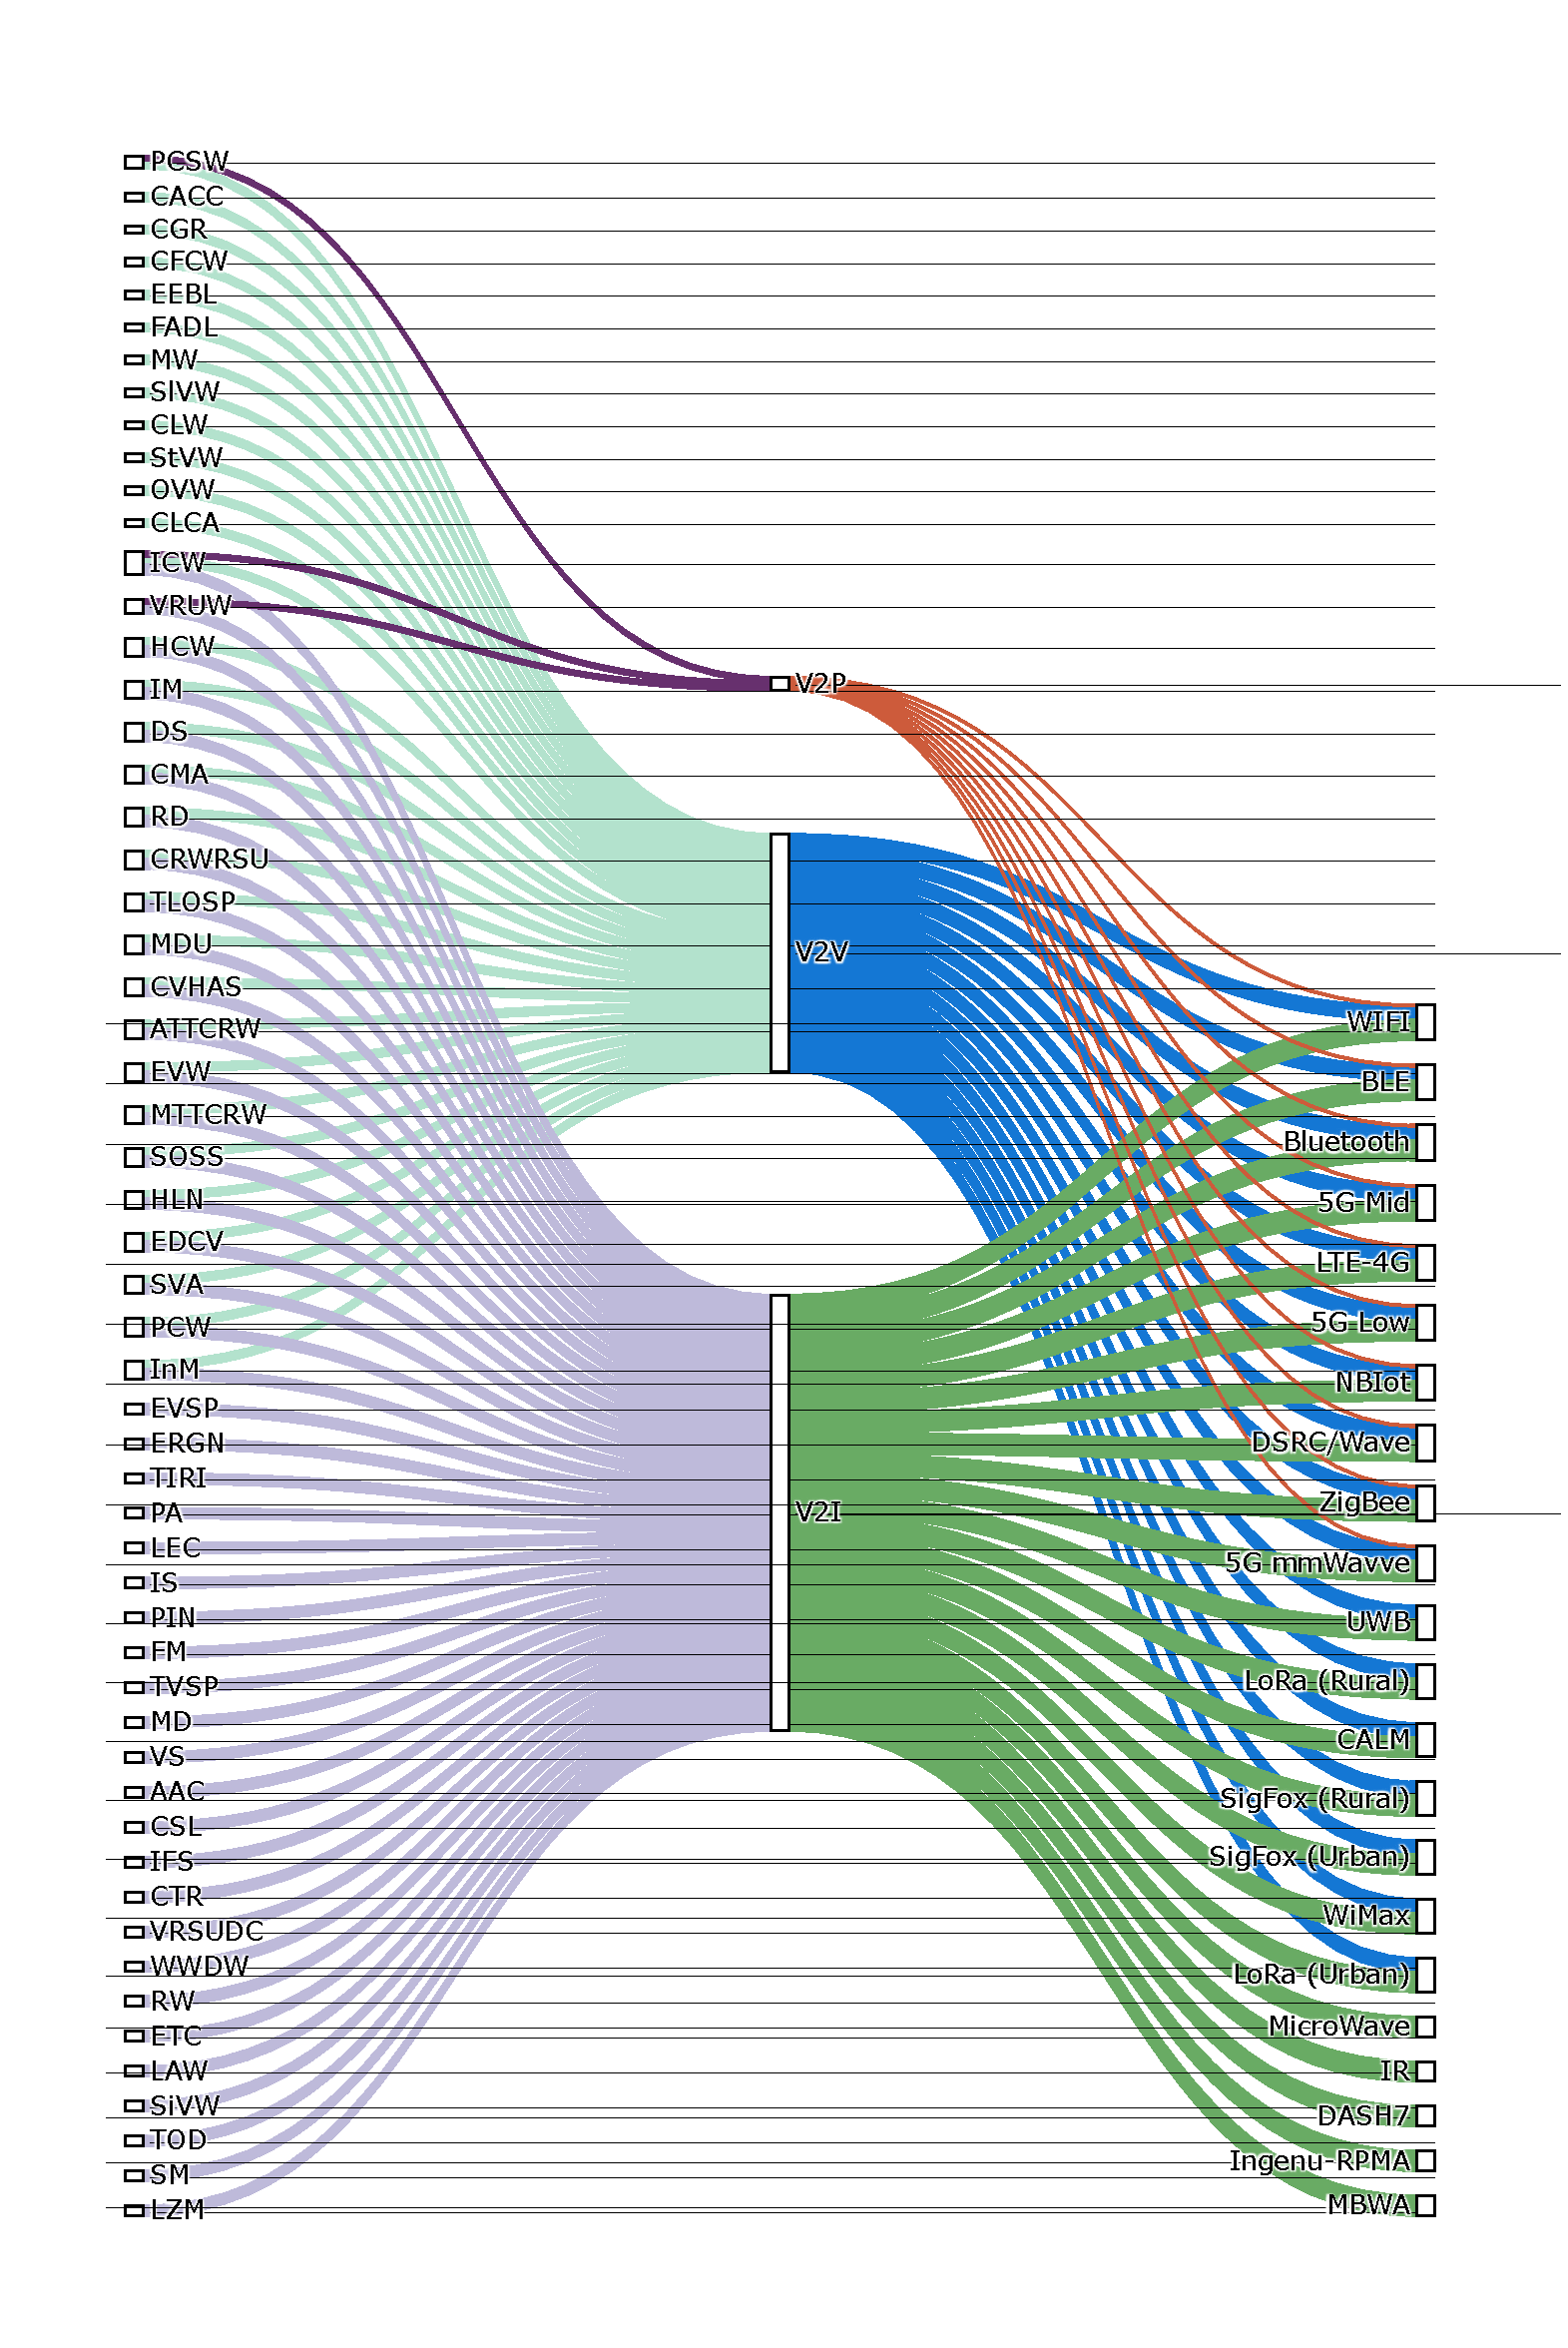
\includegraphics[width=0.9\textwidth]{merge_com_app_tech.pdf}
    \caption{Modes of communication supported by each technology and required by each application}
    \label{fig:fusion_comm}
  \end{center}
\end{figure}

The communication mode used for the operation of each application was generally found in the literature~\cite{hobert_enhancements_2015}. When this information was not readily available, it was derived from the types of road users involved by the application. 
% One of the solutions is to refer to the classification of user types which was mentioned in the transport section.
For example, for the \acrfull{VRUW} application, the \acrshort{V2P} mode is necessary. %We can also cite the pre-crash alert application which will promote V2V communication. This part first tells us about the nature of the application, namely how the application works and how the vehicle communicates in this situation. In two stages, this part allows us to acquire essential information for the last part on the merger of specific application and technologies uselable. So for all applicatin, we can represent communication mode with a Sankey on Figure~\ref{fig:fusion_comm}. 
On the other side, each communication technology can support one or more modes of communication, depending for example on the availability of devices supporting the technology for the elements of the transportation system. Finally, the applications and communication technologies can be linked as illustrated in a Sankey diagram in Figure~\ref{fig:fusion_comm}. 


\subsection{Mapping CT Applications with Communicating Technologies}

In this last section, several \acrshort{KPI}s are analyzed in order to identify the telecommunication technologies deemed to satisfy the requirements of each \acrshort{CT} applications. Not all \acrshort{KPI}s are critical and some could not be used because of a lack of information for the requirements of several applications. The mode of communication is first used to verify the suitability of communication technologies, as can be visualized in Figure~\ref{fig:fusion_comm}.  
The main \acrshort{KPI}s are latency, data rate and range. Range applies for all technologies, except for communication technologies with a dense deployment in the case of V2I communications.
% \acrshort{V2V} and \acrshort{V2I} communication modes.

%communication tech should provide data transmission with max latency, requires some amount of data transmission and to reach vehicles at least x meters away

%In this part, we are going to merge the two modes, that is to say merge the information of the communicating applications in the field of transport that we have visualized in the previous parts with the telecommunication information. This part will eventually make it possible to assimilate to each application one or more technologies that can be used for the proper functioning of this first. 

%{\bf NS: clarifier les critères utilisés pour mapper les applications et les technologies de communication, d'abord selon le mode de communications, puis quels KPI sont utilisés\\ ajouter les deux graphiques du nombre d'applications possibles par catégorie d'application et du nombre d'applications pour lequel chaque technologie peut être utilisé (segmenté par catégorie si lisible)  (2nd graphique à faire)}

%\subsubsection{Merging of modes of communication }
%In the previous section, a study to identify the modes of communication, depending on the wireless technologies and specific applications, was carried out. The first step was therefore to join this telecommunications and transport information. To evaluate applications, a Sankey can be taken into account, as in Figure~\ref{fig:fusion_comm}.

%For example, applications that only use V2P communication to operate will not consider DASH7 technologies for their operation. For example with the application of electronic emergency brake lights (EEBL), the communication is V2V vehicle type, UWB technology is unlikely to be foldable. This classification makes it possible to assign potentially usable technologies to each specific application. However, in view of this information does not take into account the performance of technologies and application requirements for proper operation. 

%{\bf HB: Clarification du mapping }
%To create the mapping, it was chosen to compare specific criteria for specific technologies and applications. The first filtering criterion is based on the mode of communication and on the range of technologies and types of application. Indeed, if the application uses V2I communications, the coverage depends on the position of the base station which is fixed and therefore no filtering is necessary for these applications. Or if the communication is V2V or V2P, the base stations are mobile so if an application needs to communicate messages to other points at a distance x, the technology must be a range y greater than X. The second filters is effects on latency, i.e. whether a technology has enough time to communicate with its environment. And the last filter was based on the data rate, which is the ability of a technology to transmit a message over a period of time. Sometimes the literature gives us this information, under it has been developed by dimensional analysis namely:

% \begin{equation}
% Data\_Rate=Message\_Frequency*Message\_Size
% \end{equation}

\begin{figure}[ht!]
  \begin{center}
    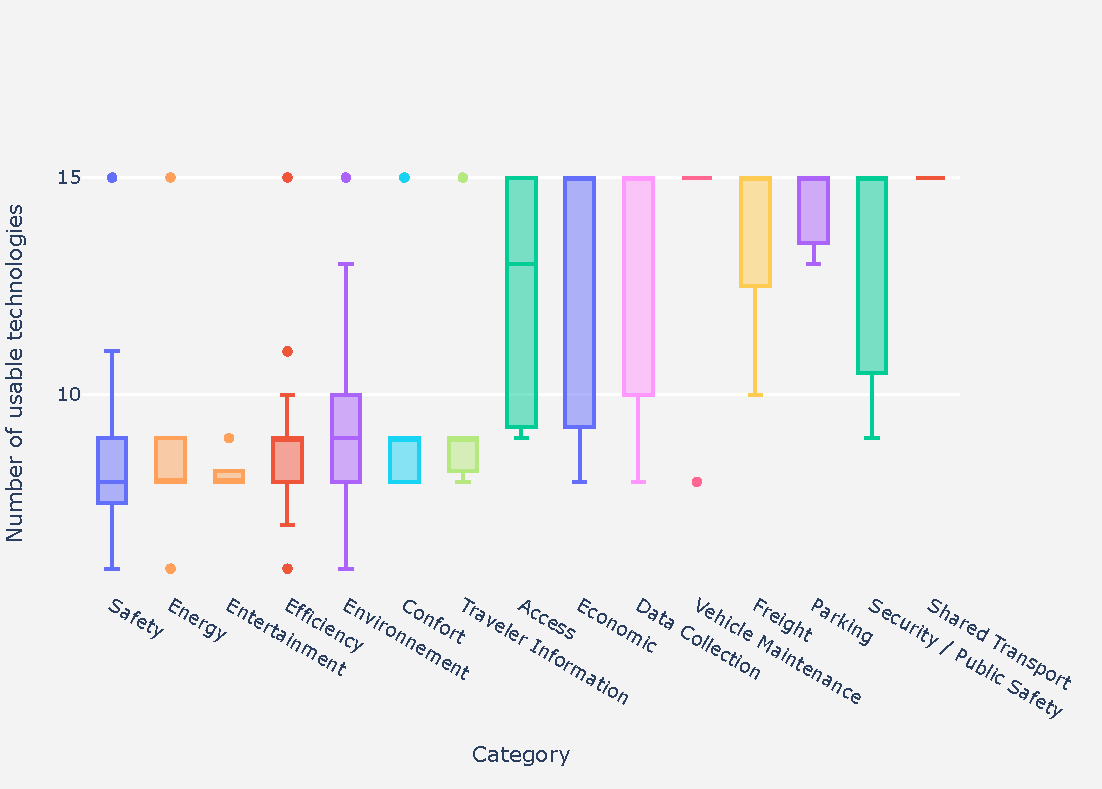
\includegraphics[width=0.9\textwidth]{box_plot.pdf}
    \caption{Distribution of the number of technologies usable by category (the boxplots show the quartiles, as well as the numbers lying outside the whiskers extending beyond the first and last quartile by 1.5 times the interquartile range).}
    \label{fig:boxplot}
  \end{center}
\end{figure}

\begin{figure}[ht!]
  \begin{center}
    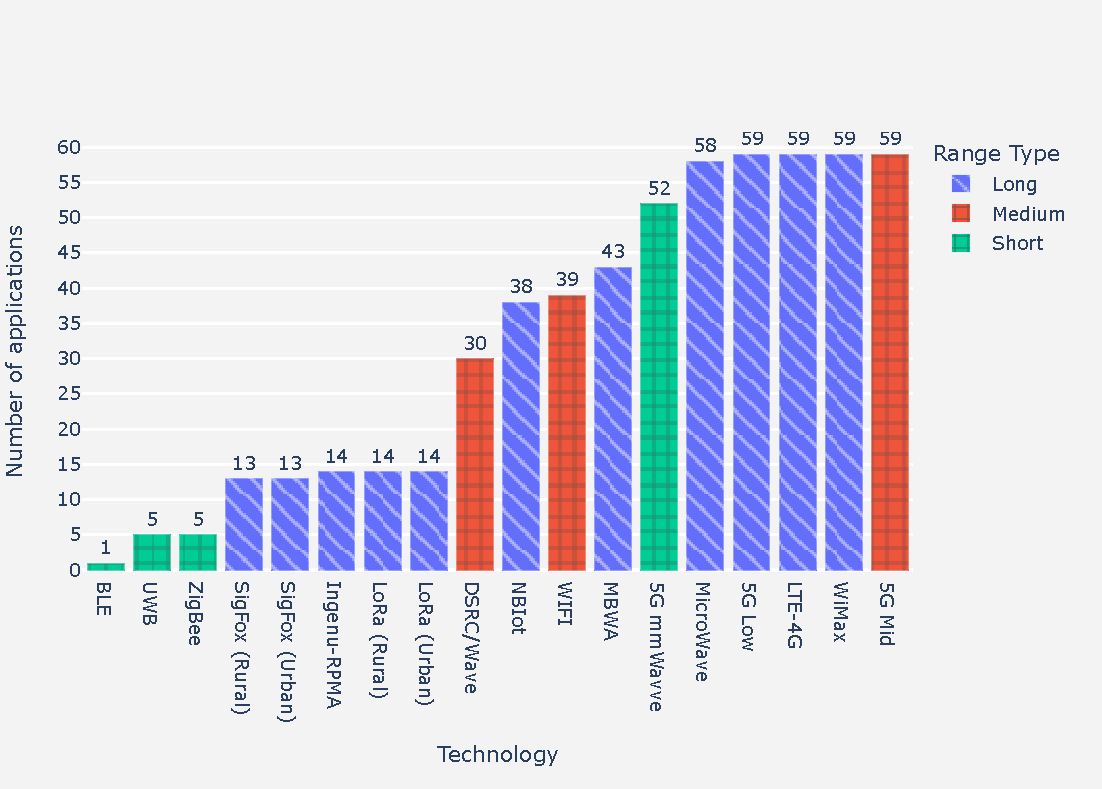
\includegraphics[width=0.9\textwidth]{bar_plot.pdf}
    \caption{Number of specific application usable by technologies.}
    \label{fig:barplot}
  \end{center}
\end{figure}

The result of the mapping can be illustrated in several ways. First, Figure~\ref{fig:boxplot} shows the distributions of the number of technologies that can be used by category, where categories are non-exclusive. It is clear that security and efficiency applications have the lowest number of suitable technologies, which is expected since they have some of the most demanding requirements, especially in terms of latency. Looking at Table~\ref{fig:techandapplong} and~\ref{fig:techandapplong2}, the technologies that can satisfy these categories are mainly 5G, 4G, NBIoT and WiMax. At the other end, the shared transport category has the most technology available to support its applications.

Second, Table~\ref{fig:table_techno} presents the proportion of applications in each category that are supported by each technology. Such a visualization provides more details than Figure~\ref{fig:boxplot} and helps identify quickly which technology to choose for a categoy or several categories of applications, apart from the all-purpose cellular technologies. 

Third, Figure~\ref{fig:barplot} represents the number of applications supported by each technology, ie.\ for which each technology can be used. Again, the clear ``winners'' are 5G and 4G technologies, along with WiMax, which can all be used for all the applications. 
%, 5G-Mid coming a close second, with the \acrfull{PCW} application being an exception because of its requirement of very low latency.
The figure also demonstrates the correlation between the range of the technology and the number of supported applications, in particular with the short range communication technologies supporting the smalled number of applications, between 1 and only 5. 5G technologies are exceptions since the short and medium range versions are expected to support all application in dense deployments to support the other uses of cellular networks. 

%{\bf NS: ajouter quelques commentaires si on ajoute le tableau des pourcentages d'applications supportees par categorie\\ conclure sur le fait que 5G est polyvalente, mais que 4G/LTE fait deja la job?} {\bf HB: Ajout de suite}
%It should be noted that WiMax and cellular technologies, with the exception of 5G mmWave, have entire uses in each category of applications.
%As can be seen in Figure ~\ref{fig:boxplot}, the Shared Transport category is the one that allows the most technologies to be developed for all of these applications. However, the categories containing the applications requiring demanding KPIs generates a reduction of their percentages of usable applications, like Entertainment applications. Finally, the short range technologies are those with the lowest percentage of applications in all categories. 

%According to the results of this taxonomy, 5G technologies merge with all the requirements of communicating applications for any category. However, based on our research, it appears that the previous generation, 4G, can also meet these requirements as well as WiMax technologies. These results also reveal that there are also a plurality of technological alternatives to the implementation of CA. However, the greater the requirements, the narrower the scope. 

\begin{landscape}
\begin{table}[ht!]
  \begin{center}
    \caption{Proportion of the applications in each category supported by each communication technology.}
    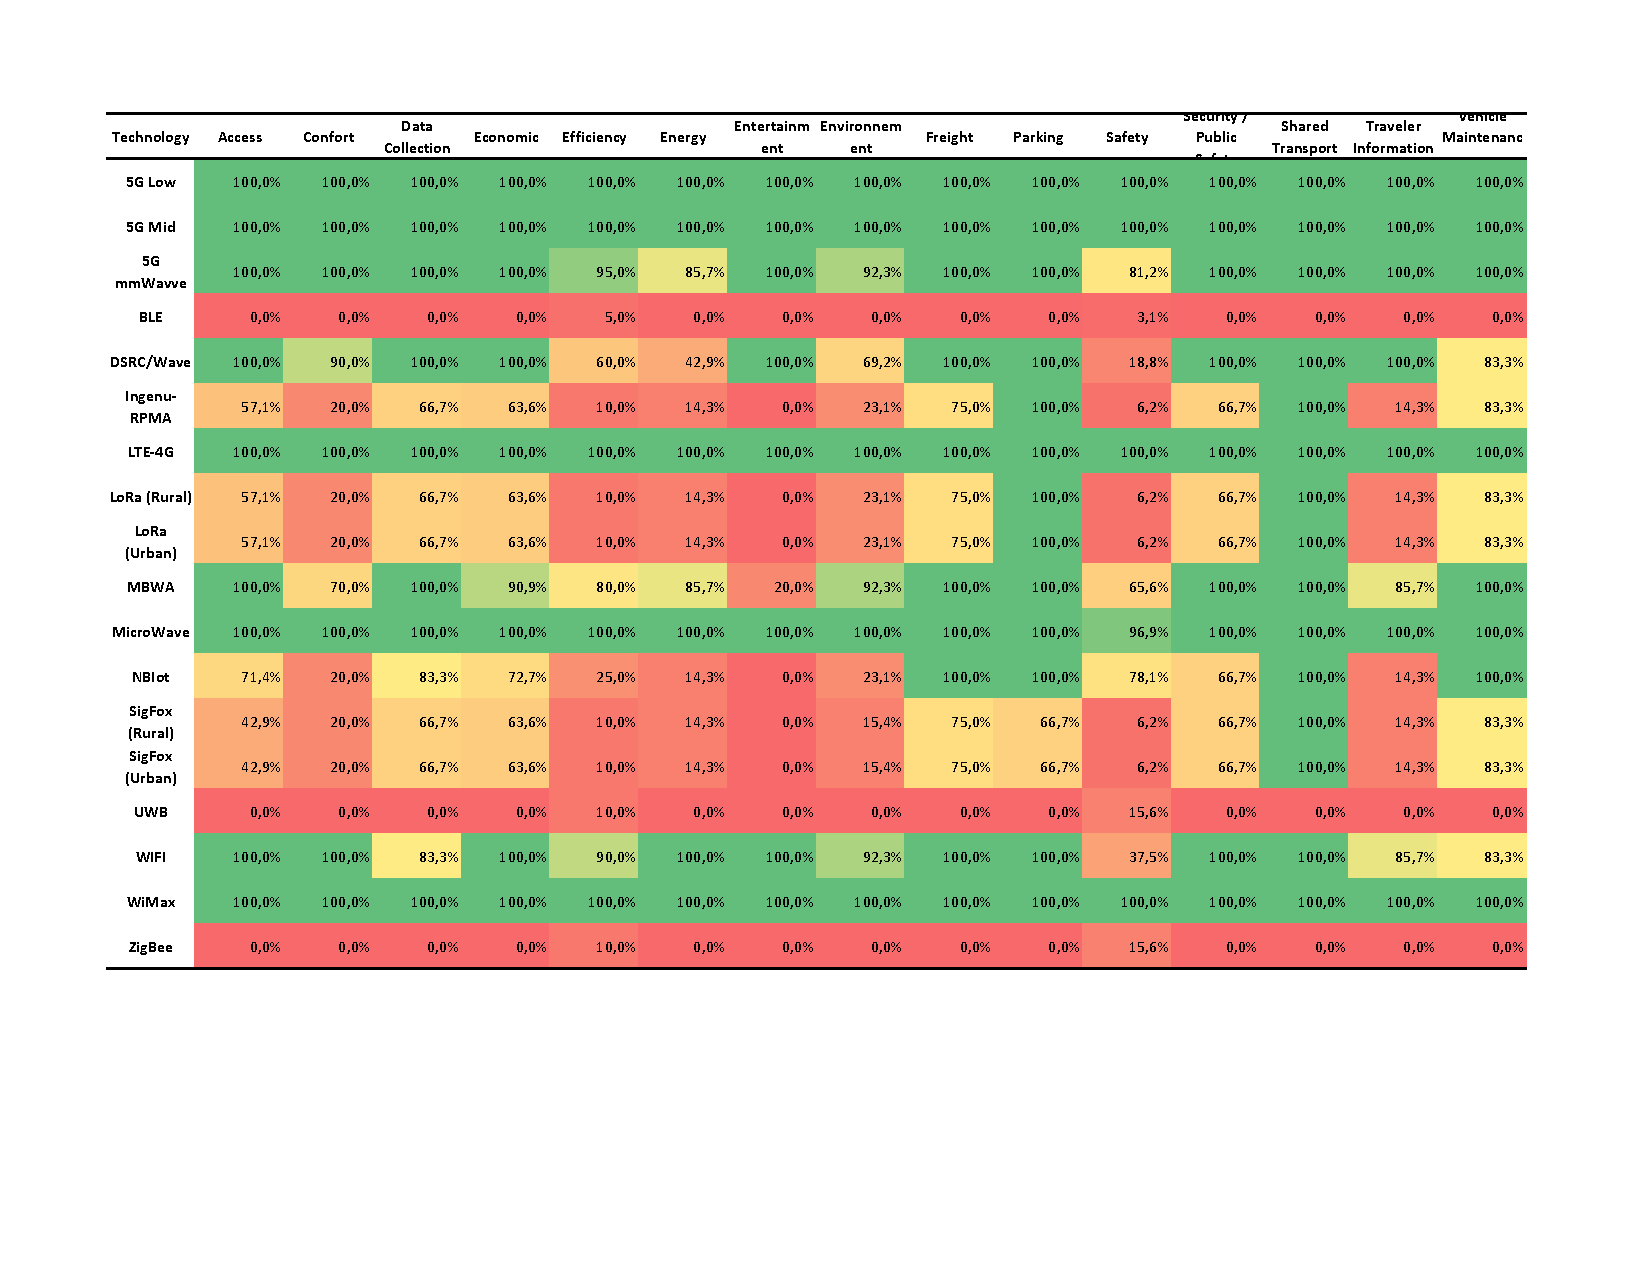
\includegraphics[width=1.5\textwidth]{tableau_percentage.pdf}
    \label{fig:table_techno}
  \end{center}
\end{table}
\end{landscape}




%By dint of the data we have collected, for this application it will seem that 5G is the most favorable for the good implementation of this application. With the following performance. Fig\ref{fig:techandapplong}\ref{fig:techandappmedium}\ref{fig:techandappshort}
%We can therefore make this deduction for other applications and thus assimilate the technologies that can be used for each application. 





\section{Conclusion}
%% Hugues

- Usefulness of this classification for a quick decision.

- Talk about the historical side, that is to say that the evolution of applications is changing. Applications that have been found in the literature for decades, the objectives are not the same. For example, insurance requests no longer go through connected cars but no longer through phones (to be verified)

- Pragmatic views on the evolution of the technologies used. That is to say that 5G is treated today but before the DRSC was more emphasized. But according to the articles, some researchers will have different paradigms, that is to say, will propose one technology rather than another.

- We have noticed in our research that most transport applications are vehicle-centric, not user-centric. One of the points for improvement in future research will surely be to take into account the multimodal aspect of this problem and not only in terms of vehicles. This paradigm will obviously pose other problems but could potentially lead to the emergence of a new type of specific application not perceived or taken into account until now.

%% NS deplace + idees
US Department of Transportation~\cite{usdt_smartphone_2020}: utiliser reference pour argumenter que les applications migrent vers d'autres plateformes, en particulier les cellulaires

Discuter la co-evolution rapide des technologies, des applications et des usages

Top-down et bottom-up

\subsection{Towards an abandonment of the DSRC?}

Since the recent announcement by the FCC in the USA of the opening of the 5.9 GHz spectrum for unlicensed uses (Wi-Fi)\cite{fcc_fcc_2020}, initially planned for the DSRC for V2X applications, the challenges of CT applications are perceived as a zero-reset problem. Notably after twenty years of research in this field with the DSRC study.

Several reasons are at the origin of this choice, apart from the costs of financing these projects and the political domain, most of the cases of applications have been confined to only experimental studies and a certain slowness persists among the automobile manufacturers to the introduction of DSRCs in new car models.

By this modification of spectrum and at the same time a possible change of paradigms in the research community, the cellular network would be a possible solution to overcome this problem. This application is called this time C-V2X for Cellular Vehicles-To-Everything, will have a spectrum reserved for automotive safety applications between 5.895 and 5.925 GHz, or 30 MHz.\cite{fcc_fcc_2020}

The United States is not the only example of this change, the European Union has proposed a bandwidth of 10 MHz, between 5.875 and 5.925 GHZ for wireless technologies, including 5G, concerning road safety using from the ETSI institute \cite{anonymous_harmonisation_2020}. Likewise for China, using 5G communication, which offers a bandwidth of 20 MHz, between 5905-5925 MHz\cite{qualcomm_c-v2x_2021}

In this new opportunity, some companies, like Ericsson\cite{ericsson_c-v2x_2021}, are working and offering solutions for applications using 4G and 5G. These companies rely on the cellular network, via IoT, to increase safety on the roads.

Despite these changes in technology and standard at the same time, the DSRC was criticized for its inactivity on the road, but the concern would it not also be the real lack of communicating car on the road? As Bezzina said, technological change will alter the architectural perspective of communication\cite{gmt_pilot_nodate} and possibly delay the implementation of CT applications. And those at the same time, the lack of a part of smart mobility for smart cities?

However, despite the difficulty of finding equivalent standards allowing cellular and DSRC technologies to operate simultaneously, there could be a hybrid architecture that favors certain applications over certain technologies.\cite{kiela_review_2020}

\subsection{The leak of applications on vehicles, the fault of the Digital Dashboard? }

The debate between the use of DSRC and the cellular network, shows a point. Most network players have as an argument the implementation of safety applications also effisiency applications. So where are the other applications, at least the categories mentioned throughout our taxonomy?

One of the possible legitimate questions in the case of automated, or even autonomous, cars is the question of the design of the Digital Dashboard for applications \cite{gowda_dashboard_2014}, in particular that of the infotainment application\cite{heikkinen_mobile_2013}.

Aside from the issues and the affectation of user driving behavior based on designs\cite{firby_its_2020}, the evolution of digital dashboards seems outdated compared to user perceptions. And they prefer to use their smartphones, which are more present on a daily basis for use.

Indeed, in addition to the aspect of form, there is the question of applications as an interaction with machines and humans. Knowing that on average a smartphone user uses only 9 applications per day\cite{web_55_2019} and especially since among the smartphone applications, on average 25\% of them are used only once\cite{noauthor__nodate}. What will happen to applications via digital dashboards?

It is also possible to see a clear difference in use between the different technologies available, which the mobile phone will potentially take priority. This is for example the case of the use of the social network Facebook in comparison between the use by the mobile phone and the desktop computers\cite{noauthor_facebook_nodate}. We can easily imagine that it could have the same depth of use with dashboards if it integrated instant messaging type applications for infoteinment.

It is therefore possible to envisage two non-exhaustive solutions to this problem. Either the car manufacturers have improved their interfaces with the driver, even if it means competing with the manufacturers of smartphones. Or companies focus on critical automotive applications, such as safety applications

Moreover, the perception of a replacement of the digital dashboard by smartphones can be considered in view of the evolution of the two designs and the percentages of use of the two technologies.\cite{abdel-aty_using_nodate}

\subsection{For more increased uses of smartphone applications?}

The previous section gives a brief overview of the evolution and influence of dashboards in certain types of applications. It should be noted that a transfer of applications to smartphones is possible as mentioned in the literature review section.

But another problem arises, over 50\% of smartphone users have downloaded apps\cite{statista_research_department_monthly_2021} and a large majority of the apps used are infotainment\cite{statista_research_department_mobile_2021}. A possible strategy for applications that are efficient or have a real impact on traffic will surely have to focus on a single application or even coexist with other infotainment applications, for example geolocation.

However, it is very likely that some applications are not usable by smartphones, such as security applications that require increased prioritization of communications, as we have seen in this taxonomy.







\appendix
\section{Definition of applications}\label{appendix:app}
\begin{enumerate}
\item \textbf{\acrfull{ATTCRW}}: This application ``informs approaching drivers/vehicles that another vehicle intends to turn across traffic'' \cite{etsi_etsi_tr_102_638_intelligent_2009,j_vehicle--vehicle_2014,al-sultan_comprehensive_2014,miucic_v2x_2018,cailean_survey_2014,xu_dsrc_2017,zeadally_tutorial_2020,noauthor_intelligent_nodate}.
\item \textbf{\acrfull{AAC}}: This application consists of an authorized vehicle transmitting its identity to access a controlled area. \cite{etsi_etsi_tr_102_638_intelligent_2009}.
\item \textbf{\acrfull{CTR}}: This application assigns to users vehicles shared or to rent and ``releases returned vehicles after collecting their reports''. \cite{etsi_etsi_tr_102_638_intelligent_2009,3gpp_tr_22886_3rd_2018}.
\item \textbf{\acrfull{CACC}}: This application provides drivers/vehicles information about the lead vehicle dynamics to improve existing \acrfull{ACC} (\acrshort{ACC} ``automatically adjusts the vehicle speed to maintain a safe distance from the lead vehicle'') ( \cite{etsi_etsi_tr_102_638_intelligent_2009,papadimitratos_vehicular_2009,brown_review_2019,zeadally_tutorial_2020,zeng_potential_2012,chang_estimated_2015,noauthor_intelligent_nodate}.
\item \textbf{\acrfull{CFCW}}: This application cooperatively detects a risk of longitudinal collision and attempts to avoid a crash either through driver assistance (information) or direct vehicle control (automated) \cite{etsi_etsi_tr_102_638_intelligent_2009,papadimitratos_vehicular_2009,brown_review_2019,boban_use_2017,3gpp_tr_22886_3rd_2018,raza_social_2018,karagiannis_vehicular_2011,chang_intelligent_2010,cailean_survey_2014, xu_dsrc_2017,bila_vehicles_2017,noauthor_5g_2015,gupta_medium_2015,dey_vehicle--vehicle_2016,xiang_research_2014,ye_v2v_2008,noauthor_intelligent_nodate}.
\item \textbf{\acrfull{CGR}}: This application allows a vehicle to ``automatically switch from high-beams to low-beams when detecting a vehicle arriving in the opposite direction \cite{etsi_etsi_tr_102_638_intelligent_2009,brown_review_2019}.
\item \textbf{\acrfull{CMA}}: This application allows drivers to negotiate together the merging process (insertion from a minor to a major road) to avoid a crash~\cite{etsi_etsi_tr_102_638_intelligent_2009,papadimitratos_vehicular_2009,j_vehicle--vehicle_2014,al-sultan_comprehensive_2014,karagiannis_vehicular_2011}.
\item \textbf{\acrfull{CVHAS}}: This application, also called ``platooning'', allows ``vehicles to operate safely as a platoon on a highway or specific lane''. \cite{etsi_etsi_tr_102_638_intelligent_2009,brown_review_2019}.
\item \textbf{\acrfull{CRWRSU}}: This application allows a \acrshort{RSU} to detect a risk of crash between two or more vehicles and to warn the drivers about this risk. \cite{etsi_etsi_tr_102_638_intelligent_2009,j_vehicle--vehicle_2014}.
\item \textbf{\acrfull{CLW}}: This application allows ``a vehicle to generate and broadcast a control-loss event to surrounding vehicles'' \cite{karagiannis_vehicular_2011}.
\item \textbf{\acrfull{EDCV}}: This application enables \acrshort{RSU}s to collect ``vehicle life cycle data for design re-use and change management''; variations of this application include the collection of ``ecologic/economic driving assistance data through exchanges between vehicles (passing by or parked)'' \cite{etsi_etsi_tr_102_638_intelligent_2009,papadimitratos_vehicular_2009,chang_estimated_2015};
\item \textbf{\acrfull{ETC}}: This application allows a \acrshort{RSU} ``to control access to a road network part after electronic toll collect'' \cite{etsi_etsi_tr_102_638_intelligent_2009,papadimitratos_vehicular_2009,brown_review_2019}.
\item \textbf{\acrfull{EEBL}}: This application corresponds to ``the switch on of emergency electronic brake lights''; the vehicle can thus ``signal its hard braking to its local followers'' to limit the risk of longitudinal crash \cite{etsi_etsi_tr_102_638_intelligent_2009,papadimitratos_vehicular_2009,brown_review_2019,j_vehicle--vehicle_2014,hamida_security_2015,boban_use_2017,etsi_tr_102_863_intelligent_2011,al-sultan_comprehensive_2014,miucic_v2x_2018,karagiannis_vehicular_2011,xu_dsrc_2017,zeadally_tutorial_2020,noauthor_intelligent_nodate}.
\item \textbf{\acrfull{EVSP}}: TODO This application uses infrastructure and communications to support emergency vehicles by sending environmental messages, especially with traffic lights. \cite{al-sultan_comprehensive_2014}
\item \textbf{\acrfull{EVW}}: This application is used to indicate the presence of an emergency vehicle to other vehicles. \cite{etsi_etsi_tr_102_638_intelligent_2009,raza_social_2018,al-sultan_comprehensive_2014,karagiannis_vehicular_2011,buchenscheit_vanet-based_2009}
\item \textbf{\acrfull{ERGN}}:This application allows a road unit to issue routes optimized according to the personalized needs of the driver. \cite{etsi_etsi_tr_102_638_intelligent_2009}
\item \textbf{\acrfull{FM}}: This application uses the vehicle collection to do fleet management. \cite{etsi_etsi_tr_102_638_intelligent_2009}
\item \textbf{\acrfull{FADL}}: This application authorizes the access of certain vehicles on a permanent or temporary basis to lanes reserved for certain cases. \cite{etsi_etsi_tr_102_638_intelligent_2009,brown_review_2019, hobert_enhancements_2015}
\item \textbf{\acrfull{GIS}}:This application allows data obtained directly through the Internet to be transmitted. \cite{karagiannis_vehicular_2011}
\item \textbf{\acrfull{HLN}}:This application allows vehicles to be informed of the presence of an object on the road. \cite{etsi_etsi_tr_102_638_intelligent_2009,papadimitratos_vehicular_2009,j_vehicle--vehicle_2014}
\item \textbf{\acrfull{HCW}}: This application makes it possible to inform vehicles traveling in the opposite direction in front of other vehicles of the risk of a head collision. \cite{karagiannis_vehicular_2011,chang_intelligent_2010,xiang_research_2014,noauthor_intelligent_nodate,ye_v2v_2008}
\item \textbf{\acrfull{IS}}: This application transmits traffic sign information to vehicles. \cite{etsi_etsi_tr_102_638_intelligent_2009}
\item \textbf{\acrfull{IM}}: This application allows instant messaging between several vehicles. \cite{etsi_etsi_tr_102_638_intelligent_2009}
%%\item \textbf{\acrfull{IFS}}: This application allows to interact with insurance and financial coverage on vehicle behavior. \cite{etsi_etsi_tr_102_638_intelligent_2009}
\item \textbf{\acrfull{ICW}}: This application consists of informing users of a risk of collision at an intersection.\cite{etsi_etsi_tr_102_638_intelligent_2009,papadimitratos_vehicular_2009,j_vehicle--vehicle_2014,al-sultan_comprehensive_2014,karagiannis_vehicular_2011,araniti_lte_2013,gupta_medium_2015,abid_pedestrian_2013}
\item \textbf{\acrfull{InM}}: This application optimizes traffic efficiency in interactions \cite{etsi_etsi_tr_102_638_intelligent_2009,papadimitratos_vehicular_2009, hobert_enhancements_2015}
\item \textbf{\acrfull{LCA}}: This application makes it possible to help a vehicle that wishes to change lane by having the status of the vehicles on the other lanes. \cite{etsi_etsi_tr_102_638_intelligent_2009,papadimitratos_vehicular_2009,brown_review_2019,boban_use_2017,al-sultan_comprehensive_2014,karagiannis_vehicular_2011,chang_intelligent_2010,cailean_survey_2014,zeadally_tutorial_2020,bila_vehicles_2017,noauthor_intelligent_nodate}
\item \textbf{\acrfull{LM}}: A DEFINIR \cite{dar_wireless_2010,noauthor_intelligent_nodate}
%\item \textbf{\acrfull{LWA}}: This application warns of restricted road conditions for vehicles and provides guidance on new routes. \cite{etsi_etsi_tr_102_638_intelligent_2009,papadimitratos_vehicular_2009}
\item \textbf{\acrfull{LZM}}: This application allows all freight agents to interact with their businesses and other users of vehicle loading and unloading. \cite{etsi_etsi_tr_102_638_intelligent_2009}
\item \textbf{\acrfull{LEC}}: This application allows vehicles and road infrastructure to make local payments for reservations and purchases. \cite{etsi_etsi_tr_102_638_intelligent_2009}
\item \textbf{\acrfull{LWZM}}: This application uses the operation of low emission zones to regulate and manage traffic in that zone. \cite{noauthor_intelligent_nodate,chang_estimated_2015}
\item \textbf{\acrfull{MDU}}: Ce cas d'utilisation permets à une unité routière de transmettre des informations topographiques au véhicules. \cite{etsi_etsi_tr_102_638_intelligent_2009,papadimitratos_vehicular_2009,noauthor_perspectives_2016,hussain_autonomous_2019}
\item \textbf{\acrlong{MD}}: This application enables the transmission of multimedia content for passenger entertainment. \cite{etsi_etsi_tr_102_638_intelligent_2009,papadimitratos_vehicular_2009,etsi_tr_102_863_intelligent_2011,xu_dsrc_2017,noauthor_perspectives_2016,gerla_vehicular_2011}
\item \textbf{\acrfull{MTTCRW}}: This application conveys information from a vehicle entering traffic and turn. \cite{etsi_etsi_tr_102_638_intelligent_2009,j_vehicle--vehicle_2014,wu_evaluation_2018}
\item \textbf{\acrfull{MW}}: This application allows vehicles to have information about the presence of a motorcycle. \cite{etsi_etsi_tr_102_638_intelligent_2009,noauthor_applications_nodate-1}
\item \textbf{\acrfull{OVW}}: This application allows an overtaking vehicle to ``signal its action to other local vehicles to secure the overtaking'' \cite{etsi_etsi_tr_102_638_intelligent_2009,j_vehicle--vehicle_2014,karagiannis_vehicular_2011,mo_simulation_2018}.
\item \textbf{\acrfull{PA}}: This application assists in the management and assistant of parking and vehicle parking demand \cite{faria_smart_2017,boban_use_2017,ferreira_self-automated_2014,noauthor_intelligent_nodate}
\item \textbf{\acrfull{PIN}}: This application informs the user of local services and points of interest. \cite{etsi_etsi_tr_102_638_intelligent_2009}
\item \textbf{\acrfull{PCW}}: A DEFINIR \cite{al-sultan_comprehensive_2014}
\item \textbf{\acrfull{PCSW}}: This application aims to ``prepare for imminent and unavoidable crash by exchanging vehicle information after unavoidable crash is detected''~\cite{etsi_etsi_tr_102_638_intelligent_2009,papadimitratos_vehicular_2009,karagiannis_vehicular_2011,chang_intelligent_2010,cailean_survey_2014,xu_dsrc_2017,sewalkar_vehicle--pedestrian_2019,zeadally_tutorial_2020,swanson_crash_2016}; % done
\item \textbf{\acrlong{CSL}}: This application allows a road infrastructure to broadcast speed limits to surrounding vehicles. \cite{etsi_etsi_tr_102_638_intelligent_2009,cailean_survey_2014, xu_dsrc_2017,noauthor_intelligent_nodate}
\item \textbf{\acrfull{RD}}: This application allows to transmit to a vehicle its diagnostic and repair notification emitter \cite{etsi_etsi_tr_102_638_intelligent_2009}
\item \textbf{\acrfull{RW}}: This application makes it possible to provide information on the state of road works and the constraints related to this state to vehicles. \cite{etsi_etsi_tr_102_638_intelligent_2009,brown_review_2019,noauthor_intelligent_nodate}
\item \textbf{\acrfull{SFONCW}}: This application allows a vehicle to communicate its abnormal and dangerous state to other vehicles. \cite{etsi_etsi_tr_102_638_intelligent_2009}
\item \textbf{\acrfull{DS}} \cite{etsi_etsi_tr_102_638_intelligent_2009}: A DEFINIR
\item \textbf{\acrfull{SiVW}}: This application allows the traffic signal violation from a user to be transmitted to vehicles. \cite{etsi_etsi_tr_102_638_intelligent_2009,papadimitratos_vehicular_2009,al-sultan_comprehensive_2014,cailean_survey_2014,xu_dsrc_2017,noauthor_intelligent_nodate}
%\item \textbf{\acrfull{SIVW}}: This application is used to communicate the presence of a slow vehicle to other vehicles that may interfere with traffic. \cite{etsi_etsi_tr_102_638_intelligent_2009,papadimitratos_vehicular_2009}
\item \textbf{\acrlong{SOSS}}: This application triggers an SOS alarm for a fatal emergency assistance request. \cite{etsi_etsi_tr_102_638_intelligent_2009,al-sultan_comprehensive_2014}
\item \textbf{\acrfull{SM}}:This application makes it possible to help a vehicle adapted to its speed to improve traffic, to make it safer and more pleasant while having an ecological and economical driving. \cite{etsi_etsi_tr_102_638_intelligent_2009,karagiannis_vehicular_2011,rakha_eco-driving_2011,xiuzheng_model_2015,noauthor_intelligent_nodate}
\item \textbf{\acrfull{StVW}}: This application consists of transmitting information to vehicles of the presence of an immobilized vehicle and which presents a danger to traffic. \cite{etsi_etsi_tr_102_638_intelligent_2009,karagiannis_vehicular_2011}
\item \textbf{\acrfull{SVA}}: This application makes it possible to transmit to the security agency a stolen vehicle \cite{etsi_etsi_tr_102_638_intelligent_2009}
\item \textbf{\acrfull{TOD}}: A DEFINIR
%\item \textbf{\acrfull{RCW}}: Ce cas d'utilisation sert à transmettre l'information d'un véhciules ou d'une station routiere de l'état du traffic à d'autres véhicules. \cite{etsi_etsi_tr_102_638_intelligent_2009,brown_review_2019,karagiannis_vehicular_2011,chang_estimated_2015}
\item \textbf{\acrfull{TIRI}}:This application informs one or more drivers of traffic conditions and suggests alternative routes in the event of congestion. \cite{etsi_etsi_tr_102_638_intelligent_2009,xu_dsrc_2017,noauthor_perspectives_2016,noauthor_intelligent_nodate}
\item \textbf{\acrfull{TLOSP}}: This application makes it possible to broadcast the status of a traffic light to approaching vehicles. \cite{etsi_etsi_tr_102_638_intelligent_2009,vandung_nguyen_efficient_2016,noauthor_intelligent_nodate}
\item \textbf{\acrfull{TVSP}}:This application enables strategic intersiton control to improve public transport services \cite{hu_transit_2014,hu_coordinated_2015,yang_implementing_2019,lee_transit_2017,zeng_potential_2012,he_multi-modal_2014}
\item \textbf{\acrfull{VRSUDC}}: This application enables software downloads for the vehicle that can potentially improve the capability or this information. \cite{etsi_etsi_tr_102_638_intelligent_2009}
\item \textbf{\acrfull{VS}}: This application uses infrastructure and automotive traffic data to update traffic status \cite{etsi_etsi_tr_102_638_intelligent_2009,boban_use_2017,raza_social_2018}
\item \textbf{\acrfull{VRUW}}: This application is used to communicate to vehicles the presence of user vulnerabilities, such as users in actives modes. \cite{etsi_etsi_tr_102_638_intelligent_2009,anaya_vulnerable_2015,raza_social_2018,al-sultan_comprehensive_2014,sewalkar_vehicle--pedestrian_2019,bila_vehicles_2017,noauthor_5g_2015,noauthor_intelligent_nodate,zeng_potential_2012,boban_use_2017}
\item \textbf{\acrfull{WWDW}}: This application allows information to be transmitted to vehicles when another vehicle is present in the wrong direction. \cite{etsi_etsi_tr_102_638_intelligent_2009,karagiannis_vehicular_2011,zeng_potential_2012,vogel_cloud-based_2017}
\end{enumerate}


\section{Acronyms}
\printnoidxglossary[type=\acronymtype]
%\section{Definition of the applications}


% \begin{figure*}[ht!]
%   \begin{center}
%     \includegraphics[width=11cm]{road_type.png}
%     \caption{Road Type Application}
%     \label{fig:road_type}
%   \end{center}
% \end{figure*}



% \begin{figure*}[ht!]
%   \begin{center}
%     \includegraphics[width=11cm]{application_mecanisme.png}
%     \caption{Mecanisme Application}
%     \label{fig:application_mecanisme}
%   \end{center}
% \end{figure*}



% \begin{figure*}[ht!]
%   \begin{center}

%     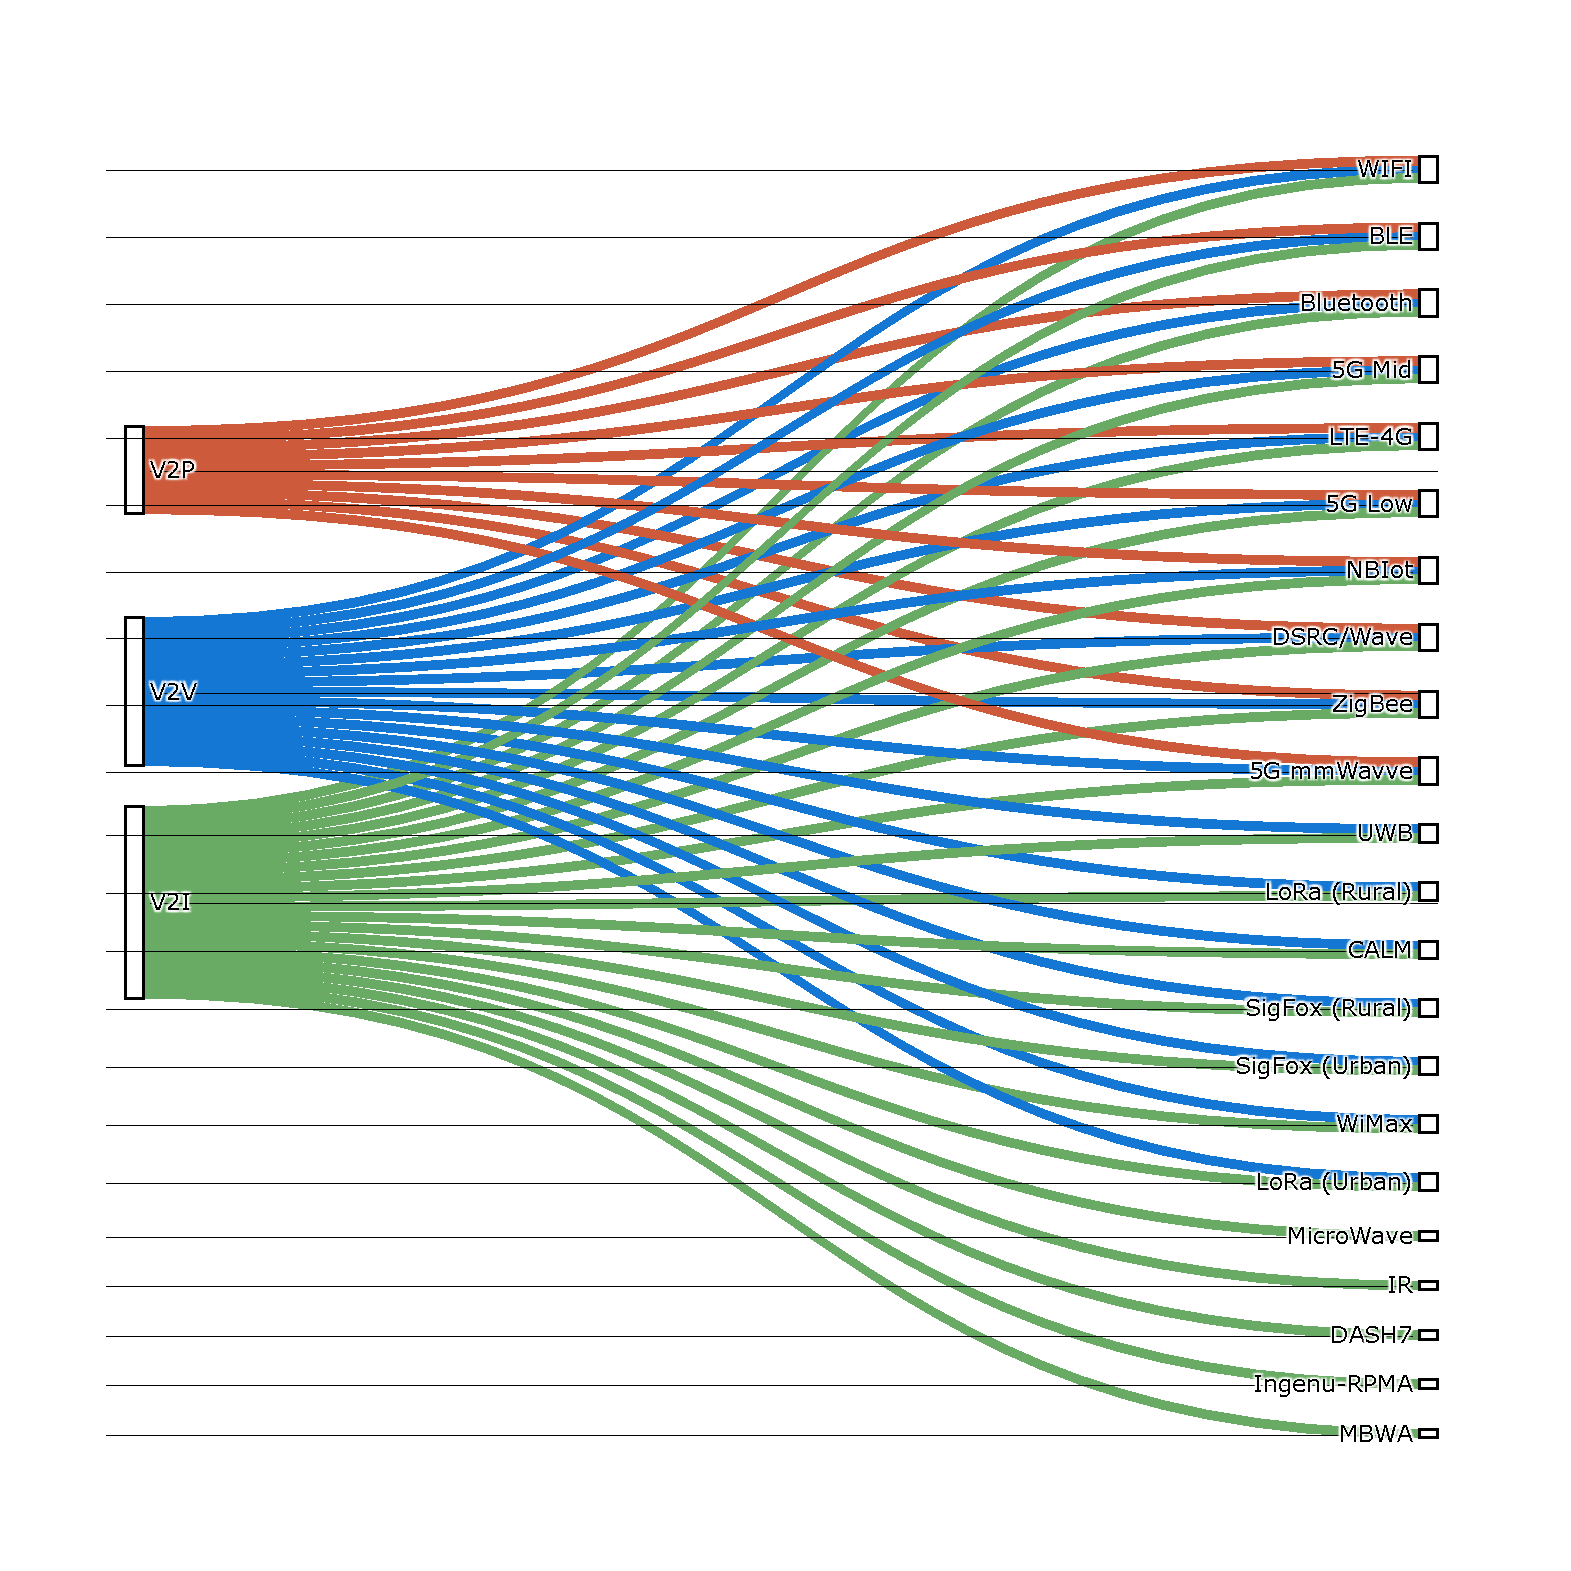
\includegraphics[width=16cm]{communication_mode_technologies.pdf}
%     \caption{mode of communication of each technology}
%     \label{fig:mode-com-tech}
%   \end{center}
% \end{figure*}


% \begin{figure*}[ht!]
%   \begin{center}
%     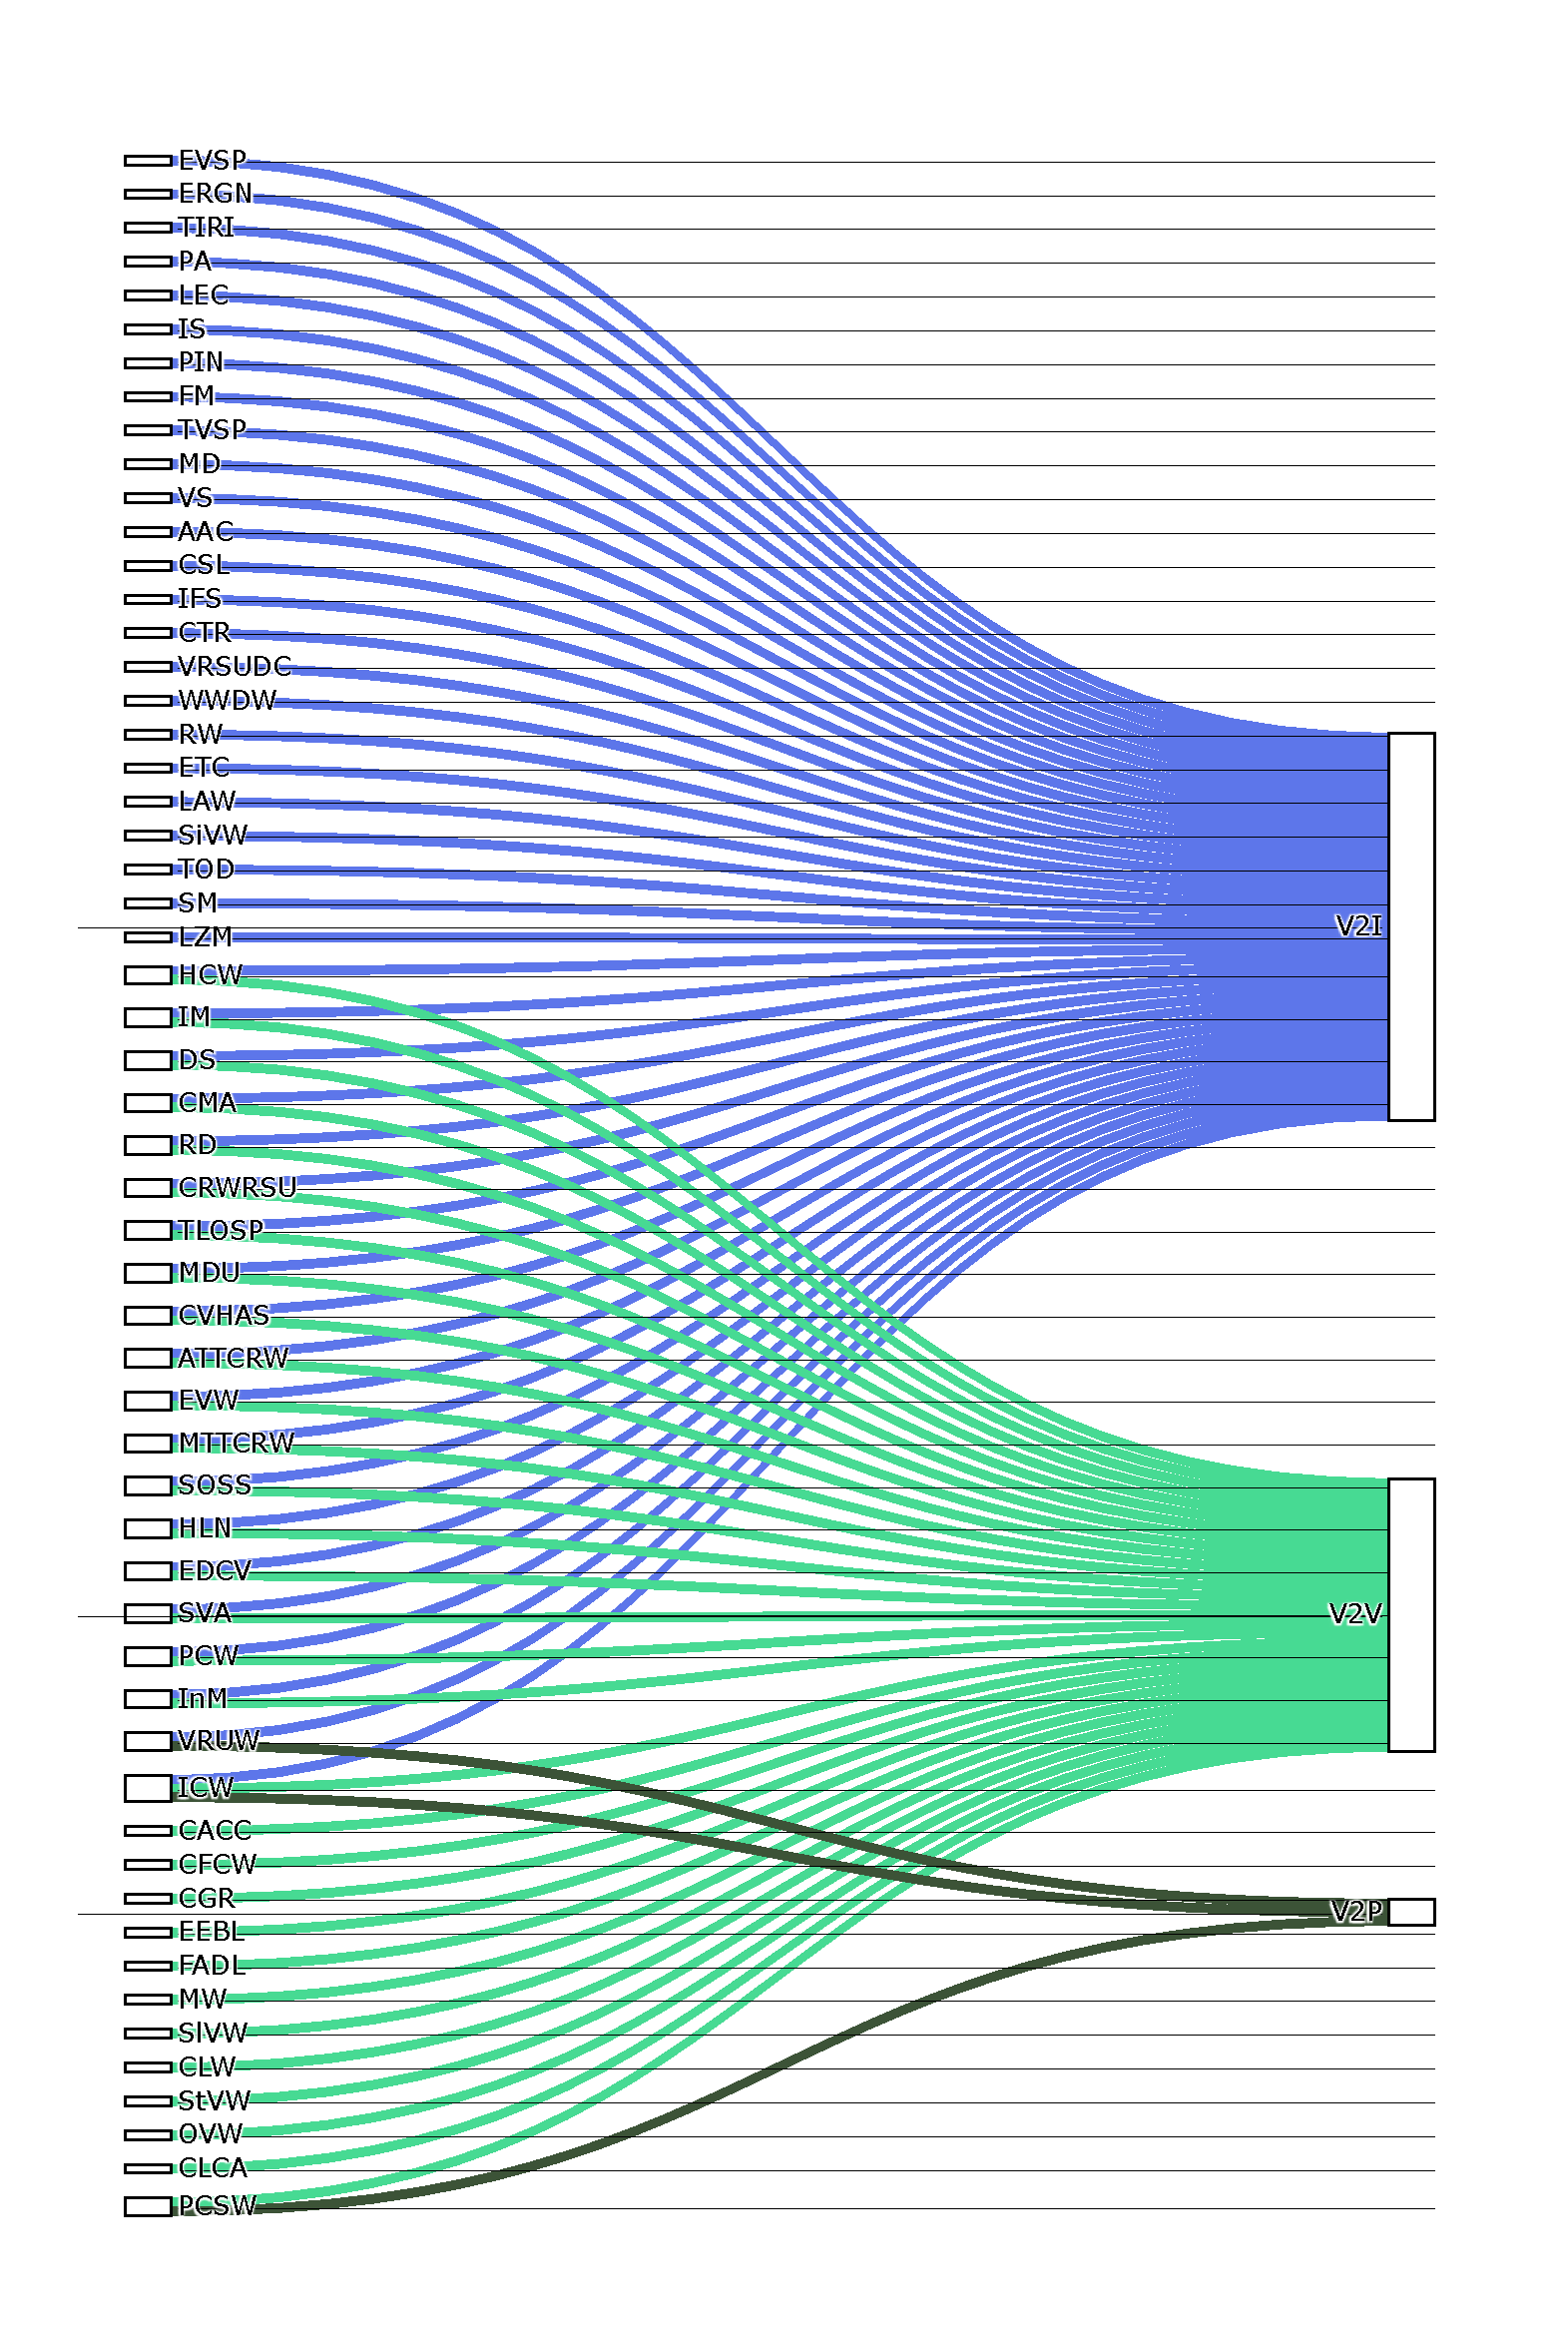
\includegraphics[width=15.5cm]{application_communication_mode.pdf}
%     \caption{mode of communication of application}
%     \label{fig:mode-com-app}
% \end{center}
% \end{figure*}





% \begin{figure*}[ht!]
%   \begin{center}
%     \includegraphics[width=17cm]{latencypriority.png}
%     \caption{Latency and priority of application}
%     \label{fig:latency-priority}
%   \end{center}
% \end{figure*}



% \begin{figure*}[ht!]
% \centering
% \subfloat[Access]{\includegraphics[width=0.55\textwidth]{para_coor/access.png}}
% \subfloat[Confort]{\includegraphics[width=0.55\textwidth]{para_coor/confort.png}}
% \end{figure*}
% \begin{figure*}[ht!]
% \ContinuedFloat
% \centering
% \subfloat[Data collection]{\includegraphics[width=0.55\textwidth]{para_coor/data_collection.png}}
% \subfloat[Economical]{\includegraphics[width=0.55\textwidth]{para_coor/economical.png}}
% \end{figure*}
% \begin{figure*}[ht!]
% \ContinuedFloat
% \centering
% \subfloat[Efficiency]{\includegraphics[width=0.55\textwidth]{para_coor/efficiency.png}}
% \subfloat[Energy]{\includegraphics[width=0.55\textwidth]{para_coor/energy.png}}
% \end{figure*}
% \begin{figure*}[ht!]
% \ContinuedFloat
% \centering
% \subfloat[Entertainment]{\includegraphics[width=0.55\textwidth]{para_coor/entertainment.png}}
% \subfloat[Environnement]{\includegraphics[width=0.55\textwidth]{para_coor/enviro.png}}
% \end{figure*}
% \begin{figure*}[ht!]
% \ContinuedFloat
% \centering
% \subfloat[Freight]{\includegraphics[width=0.55\textwidth]{para_coor/freight.png}}
% \subfloat[Parking]{\includegraphics[width=0.55\textwidth]{para_coor/parking.png}}
% \end{figure*}
% \begin{figure*}[ht!]
% \ContinuedFloat
% \centering
% \subfloat[Safety]{\includegraphics[width=0.55\textwidth]{para_coor/safety.png}}
% \subfloat[Security]{\includegraphics[width=0.55\textwidth]{para_coor/security.png}}
% \end{figure*}
% \begin{figure*}[ht!]
% \ContinuedFloat
% \centering
% \subfloat[Shared Transport]{\includegraphics[width=0.55\textwidth]{para_coor/shared_transport.png}}
% \subfloat[Travel Information]{\includegraphics[width=0.55\textwidth]{para_coor/travel_information.png}}
% \end{figure*}
% \begin{figure*}[ht!]
% \ContinuedFloat
% \centering
% \subfloat[Vehicule Maitenance]{\includegraphics[width=0.55\textwidth]{para_coor/vehicle_maitenance.png}}
% \caption{Parallel coordinates Category KPI}
% \end{figure*}

%\FloatBarrier

\begin{table}[ht!]
\centering
\caption{Long Range and application - A}
    \label{fig:techandapplong}
\begin{tabular}{lcccccccc}
\hline
\textbf{Application} & \textbf{5G Low} & \textbf{5G Mid} & \textbf{5G mmWavve} & \textbf{DASH7} & \textbf{Ingenu-RPMA} & \textbf{LoRa (Rural)} & \textbf{LoRa (Urban)} & \textbf{LTE-4G} \\
\hline
\textbf{AAC}         & Yes             & Yes             & -                   & Yes            & Yes                  & Yes                   & Yes                   & Yes             \\
\textbf{ATTCRW}      & Yes             & Yes             & -                   & -              & -                    & -                     & -                     & Yes             \\
\textbf{CACC}        & Yes             & Yes             & -                   & -              & -                    & -                     & -                     & Yes             \\
\textbf{CFCW}        & Yes             & Yes             & -                   & -              & -                    & -                     & -                     & Yes             \\
\textbf{CGR}         & Yes             & Yes             & Yes                 & -              & -                    & -                     & -                     & Yes             \\
\textbf{CLCA}        & Yes             & Yes             & -                   & -              & -                    & -                     & -                     & Yes             \\
\textbf{CLW}         & Yes             & Yes             & -                   & -              & -                    & -                     & -                     & Yes             \\
\textbf{CMA}         & Yes             & Yes             & -                   & -              & -                    & -                     & -                     & Yes             \\
\textbf{CRWRSU}      & Yes             & Yes             & -                   & -              & -                    & -                     & -                     & Yes             \\
\textbf{CSL}         & Yes             & Yes             & -                   & -              & -                    & -                     & -                     & Yes             \\
\textbf{CTR}         & Yes             & Yes             & -                   & Yes            & Yes                  & Yes                   & Yes                   & Yes             \\
\textbf{CVHAS}       & Yes             & Yes             & -                   & -              & -                    & -                     & -                     & Yes             \\
\textbf{DS}          & Yes             & Yes             & -                   & Yes            & Yes                  & Yes                   & Yes                   & Yes             \\
\textbf{EDCV}        & Yes             & Yes             & -                   & Yes            & Yes                  & Yes                   & Yes                   & Yes             \\
\textbf{EEBL}        & Yes             & Yes             & -                   & -              & -                    & -                     & -                     & Yes             \\
\textbf{ERGN}        & Yes             & Yes             & -                   & Yes            & Yes                  & Yes                   & Yes                   & Yes             \\
\textbf{ETC}         & Yes             & Yes             & -                   & -              & -                    & -                     & -                     & Yes             \\
\textbf{EVSP}        & Yes             & Yes             & -                   & Yes            & Yes                  & Yes                   & Yes                   & Yes             \\
\textbf{EVW}         & Yes             & Yes             & -                   & -              & -                    & -                     & -                     & Yes             \\
\textbf{FADL}        & Yes             & Yes             & -                   & -              & -                    & Yes                   & Yes                   & Yes             \\
\textbf{FM}          & Yes             & Yes             & -                   & Yes            & Yes                  & Yes                   & Yes                   & Yes             \\
\textbf{HCW}         & Yes             & Yes             & -                   & -              & -                    & -                     & -                     & Yes             \\
\textbf{HLN}         & Yes             & Yes             & -                   & -              & -                    & -                     & -                     & Yes             \\
\textbf{ICW}         & Yes             & Yes             & -                   & -              & -                    & -                     & -                     & Yes             \\
\textbf{IFS}         & Yes             & Yes             & -                   & Yes            & Yes                  & Yes                   & Yes                   & Yes             \\
\textbf{IM}          & Yes             & Yes             & -                   & Yes            & Yes                  & Yes                   & Yes                   & Yes             \\
\textbf{InM}         & Yes             & Yes             & -                   & Yes            & Yes                  & Yes                   & Yes                   & Yes             \\
\textbf{IS}          & Yes             & Yes             & -                   & Yes            & Yes                  & Yes                   & Yes                   & Yes             \\
\textbf{LAW}         & Yes             & Yes             & -                   & Yes            & Yes                  & Yes                   & Yes                   & Yes             \\
\textbf{LEC}         & Yes             & Yes             & -                   & Yes            & Yes                  & Yes                   & Yes                   & Yes             \\
\textbf{LZM}         & Yes             & Yes             & -                   & Yes            & Yes                  & Yes                   & Yes                   & Yes             \\
\textbf{MD}          & Yes             & Yes             & -                   & Yes            & Yes                  & Yes                   & Yes                   & Yes             \\
\textbf{MDU}         & Yes             & Yes             & -                   & Yes            & Yes                  & Yes                   & Yes                   & Yes             \\
\textbf{MTTCRW}      & Yes             & Yes             & -                   & -              & -                    & -                     & -                     & Yes             \\
\textbf{MW}          & Yes             & Yes             & Yes                 & -              & -                    & -                     & -                     & Yes             \\
\textbf{OVW}         & Yes             & Yes             & -                   & -              & -                    & -                     & -                     & Yes             \\
\textbf{PA}          & Yes             & Yes             & -                   & Yes            & Yes                  & Yes                   & Yes                   & Yes             \\
\textbf{PCSW}        & Yes             & Yes             & Yes                 & -              & -                    & -                     & -                     & Yes             \\
\textbf{PCW}         & Yes             & -               & -                   & -              & -                    & -                     & -                     & Yes             \\
\textbf{PIN}         & Yes             & Yes             & -                   & Yes            & Yes                  & Yes                   & Yes                   & Yes             \\
\textbf{RD}          & Yes             & Yes             & -                   & Yes            & Yes                  & Yes                   & Yes                   & Yes             \\
\textbf{RW}          & Yes             & Yes             & -                   & -              & -                    & -                     & -                     & Yes             \\
\textbf{SiVW}        & Yes             & Yes             & -                   & -              & -                    & -                     & -                     & Yes             \\
\textbf{SlVW}        & Yes             & Yes             & Yes                 & -              & -                    & -                     & -                     & Yes             \\
\textbf{SM}          & Yes             & Yes             & -                   & Yes            & Yes                  & Yes                   & Yes                   & Yes             \\
\textbf{SOSS}        & Yes             & Yes             & -                   & Yes            & Yes                  & Yes                   & Yes                   & Yes             \\
\textbf{StVW}        & Yes             & Yes             & -                   & -              & -                    & -                     & -                     & Yes             \\
\textbf{SVA}         & Yes             & Yes             & -                   & Yes            & Yes                  & Yes                   & Yes                   & Yes             \\
\textbf{TIRI}        & Yes             & Yes             & -                   & Yes            & Yes                  & Yes                   & Yes                   & Yes             \\
\textbf{TLOSP}       & Yes             & Yes             & -                   & -              & -                    & -                     & -                     & Yes             \\
\textbf{TOD}         & Yes             & Yes             & -                   & -              & -                    & -                     & -                     & Yes             \\
\textbf{TVSP}        & Yes             & Yes             & -                   & Yes            & Yes                  & Yes                   & Yes                   & Yes             \\
\textbf{VRSUDC}      & Yes             & Yes             & -                   & Yes            & Yes                  & Yes                   & Yes                   & Yes             \\
\textbf{VRUW}        & Yes             & Yes             & Yes                 & -              & -                    & -                     & -                     & Yes             \\
\textbf{VS}          & Yes             & Yes             & -                   & Yes            & Yes                  & Yes                   & Yes                   & Yes             \\
\textbf{WWDW}        & Yes             & Yes             & -                   & -              & -                    & -                     & -                     & Yes            \\
\hline
\end{tabular}
\end{table}

\FloatBarrier
\begin{table}[ht!]
\centering
\caption{Long Range and application - B}
\begin{tabular}{lcccccc}
\hline
\textbf{Application} & \textbf{MBWA} & \textbf{MicroWave} & \textbf{NBIot} & \textbf{SigFox (Rural)} & \textbf{SigFox (Urban)} & \textbf{WiMax} \\
\hline
\textbf{AAC}         & Yes           & Yes                & Yes            & Yes                     & Yes                     & Yes            \\
\textbf{ATTCRW}      & Yes           & Yes                & Yes            & -                       & -                       & Yes            \\
\textbf{CACC}        & -             & -                  & Yes            & -                       & -                       & Yes            \\
\textbf{CFCW}        & -             & -                  & Yes            & -                       & -                       & Yes            \\
\textbf{CGR}         & -             & -                  & Yes            & -                       & -                       & Yes            \\
\textbf{CLCA}        & -             & -                  & Yes            & -                       & -                       & Yes            \\
\textbf{CLW}         & -             & -                  & Yes            & -                       & -                       & Yes            \\
\textbf{CMA}         & Yes           & Yes                & Yes            & -                       & -                       & Yes            \\
\textbf{CRWRSU}      & Yes           & Yes                & Yes            & -                       & -                       & Yes            \\
\textbf{CSL}         & Yes           & Yes                & Yes            & -                       & -                       & Yes            \\
\textbf{CTR}         & Yes           & Yes                & Yes            & Yes                     & Yes                     & Yes            \\
\textbf{CVHAS}       & Yes           & Yes                & Yes            & -                       & -                       & Yes            \\
\textbf{DS}          & Yes           & Yes                & Yes            & Yes                     & Yes                     & Yes            \\
\textbf{EDCV}        & Yes           & Yes                & Yes            & Yes                     & Yes                     & Yes            \\
\textbf{EEBL}        & -             & -                  & Yes            & -                       & -                       & Yes            \\
\textbf{ERGN}        & Yes           & Yes                & Yes            & Yes                     & Yes                     & Yes            \\
\textbf{ETC}         & Yes           & Yes                & Yes            & -                       & -                       & Yes            \\
\textbf{EVSP}        & Yes           & Yes                & Yes            & Yes                     & Yes                     & Yes            \\
\textbf{EVW}         & Yes           & Yes                & Yes            & -                       & -                       & Yes            \\
\textbf{FADL}        & -             & -                  & Yes            & Yes                     & Yes                     & Yes            \\
\textbf{FM}          & Yes           & Yes                & Yes            & Yes                     & Yes                     & Yes            \\
\textbf{HCW}         & Yes           & Yes                & Yes            & -                       & -                       & Yes            \\
\textbf{HLN}         & Yes           & Yes                & Yes            & -                       & -                       & Yes            \\
\textbf{ICW}         & Yes           & Yes                & Yes            & -                       & -                       & Yes            \\
\textbf{IFS}         & Yes           & Yes                & Yes            & Yes                     & Yes                     & Yes            \\
\textbf{IM}          & Yes           & Yes                & Yes            & Yes                     & Yes                     & Yes            \\
\textbf{InM}         & Yes           & Yes                & Yes            & Yes                     & Yes                     & Yes            \\
\textbf{IS}          & Yes           & Yes                & Yes            & Yes                     & Yes                     & Yes            \\
\textbf{LAW}         & Yes           & Yes                & Yes            & Yes                     & Yes                     & Yes            \\
\textbf{LEC}         & Yes           & Yes                & Yes            & Yes                     & Yes                     & Yes            \\
\textbf{LZM}         & Yes           & Yes                & Yes            & Yes                     & Yes                     & Yes            \\
\textbf{MD}          & Yes           & Yes                & Yes            & Yes                     & Yes                     & Yes            \\
\textbf{MDU}         & Yes           & Yes                & Yes            & Yes                     & Yes                     & Yes            \\
\textbf{MTTCRW}      & Yes           & Yes                & Yes            & -                       & -                       & Yes            \\
\textbf{MW}          & -             & -                  & Yes            & -                       & -                       & Yes            \\
\textbf{OVW}         & -             & -                  & Yes            & -                       & -                       & Yes            \\
\textbf{PA}          & Yes           & Yes                & Yes            & Yes                     & Yes                     & Yes            \\
\textbf{PCSW}        & -             & -                  & -              & -                       & -                       & Yes            \\
\textbf{PCW}         & Yes           & Yes                & Yes            & -                       & -                       & Yes            \\
\textbf{PIN}         & Yes           & Yes                & Yes            & Yes                     & Yes                     & Yes            \\
\textbf{RD}          & Yes           & Yes                & Yes            & Yes                     & Yes                     & Yes            \\
\textbf{RW}          & Yes           & Yes                & Yes            & -                       & -                       & Yes            \\
\textbf{SiVW}        & Yes           & Yes                & Yes            & -                       & -                       & Yes            \\
\textbf{SlVW}        & -             & -                  & Yes            & -                       & -                       & Yes            \\
\textbf{SM}          & Yes           & Yes                & Yes            & Yes                     & Yes                     & Yes            \\
\textbf{SOSS}        & Yes           & Yes                & Yes            & Yes                     & Yes                     & Yes            \\
\textbf{StVW}        & -             & -                  & Yes            & -                       & -                       & Yes            \\
\textbf{SVA}         & Yes           & Yes                & Yes            & Yes                     & Yes                     & Yes            \\
\textbf{TIRI}        & Yes           & Yes                & Yes            & Yes                     & Yes                     & Yes            \\
\textbf{TLOSP}       & Yes           & Yes                & Yes            & -                       & -                       & Yes            \\
\textbf{TOD}         & Yes           & Yes                & Yes            & -                       & -                       & Yes            \\
\textbf{TVSP}        & Yes           & Yes                & Yes            & Yes                     & Yes                     & Yes            \\
\textbf{VRSUDC}      & Yes           & Yes                & Yes            & Yes                     & Yes                     & Yes            \\
\textbf{VRUW}        & Yes           & Yes                & Yes            & -                       & -                       & Yes            \\
\textbf{VS}          & Yes           & Yes                & Yes            & Yes                     & Yes                     & Yes            \\
\textbf{WWDW}        & Yes           & Yes                & Yes            & -                       & -                       & Yes           \\
\hline
\end{tabular}
\end{table}

\FloatBarrier
\begin{table}[ht!]
\centering
\caption{Medium Range and application }
    \label{fig:techandappmedium}
\begin{tabular}{lcc}
\hline
\textbf{Application} & \textbf{DSRC/Wave} & \textbf{WIFI} \\
\hline
\textbf{AAC}                  & Yes                & Yes           \\
\textbf{ATTCRW}               & -                  & -             \\
\textbf{CACC}                 & -                  & Yes           \\
\textbf{CFCW}                 & -                  & Yes           \\
\textbf{CGR}                  & -                  & Yes           \\
\textbf{CLCA}                 & -                  & -             \\
\textbf{CLW}                  & -                  & -             \\
\textbf{CMA}                  & -                  & -             \\
\textbf{CRWRSU}               & -                  & -             \\
\textbf{CSL}                  & -                  & Yes           \\
\textbf{CTR}                  & Yes                & Yes           \\
\textbf{CVHAS}                & -                  & Yes           \\
\textbf{DS}                   & Yes                & -             \\
\textbf{EDCV}                 & Yes                & Yes           \\
\textbf{EEBL}                 & -                  & -             \\
\textbf{ERGN}                 & Yes                & Yes           \\
\textbf{ETC}                  & Yes                & Yes           \\
\textbf{EVSP}                 & Yes                & Yes           \\
\textbf{EVW}                  & -                  & -             \\
\textbf{FADL}                 & Yes                & Yes           \\
\textbf{FM}                   & Yes                & Yes           \\
\textbf{HCW}                  & -                  & -             \\
\textbf{HLN}                  & -                  & -             \\
\textbf{ICW}                  & -                  & -             \\
\textbf{IFS}                  & Yes                & Yes           \\
\textbf{IM}                   & Yes                & Yes           \\
\textbf{InM}                  & Yes                & Yes           \\
\textbf{IS}                   & Yes                & Yes           \\
\textbf{LAW}                  & Yes                & Yes           \\
\textbf{LEC}                  & Yes                & Yes           \\
\textbf{LZM}                  & Yes                & Yes           \\
\textbf{MD}                   & Yes                & Yes           \\
\textbf{MDU}                  & Yes                & Yes           \\
\textbf{MTTCRW}               & -                  & -             \\
\textbf{MW}                   & -                  & Yes           \\
\textbf{OVW}                  & -                  & -             \\
\textbf{PA}                   & Yes                & Yes           \\
\textbf{PCSW}                 & -                  & -             \\
\textbf{PCW}                  & -                  & -             \\
\textbf{PIN}                  & Yes                & Yes           \\
\textbf{RD}                   & Yes                & Yes           \\
\textbf{RW}                   & -                  & -             \\
\textbf{SiVW}                 & -                  & -             \\
\textbf{SlVW}                 & -                  & Yes           \\
\textbf{SM}                   & Yes                & Yes           \\
\textbf{SOSS}                 & Yes                & Yes           \\
\textbf{StVW}                 & -                  & -             \\
\textbf{SVA}                  & Yes                & Yes           \\
\textbf{TIRI}                 & Yes                & Yes           \\
\textbf{TLOSP}                & -                  & Yes           \\
\textbf{TOD}                  & -                  & Yes           \\
\textbf{TVSP}                 & Yes                & Yes           \\
\textbf{VRSUDC}               & Yes                & Yes           \\
\textbf{VRUW}                 & -                  & Yes           \\
\textbf{VS}                   & Yes                & Yes           \\
\textbf{WWDW}                 & -                  & -             \\
\hline
\end{tabular}
\end{table}

\FloatBarrier
\begin{table}[ht!]
\centering
\caption{Short Range and application }
    \label{fig:techandappshort}
\begin{tabular}{lcccc}
\hline
\textbf{Applications}  & \textbf{Bluetooth} & \textbf{BLE} & \textbf{UWB} & \textbf{ZigBee} \\
\hline
\textbf{AAC}           & -                  & -            & -            & -               \\
\textbf{ATTCRW}        & -                  & -            & -            & -               \\
\textbf{CACC}          & -                  & -            & -            & -               \\
\textbf{CFCW}          & -                  & -            & -            & -               \\
\textbf{CGR}           & -                  & Yes          & Yes          & Yes             \\
\textbf{CLCA}          & -                  & -            & -            & -               \\
\textbf{CLW}           & -                  & -            & -            & -               \\
\textbf{CMA}           & -                  & -            & -            & -               \\
\textbf{CRWRSU}        & -                  & -            & -            & -               \\
\textbf{CSL}           & -                  & -            & -            & -               \\
\textbf{CTR}           & -                  & -            & -            & -               \\
\textbf{CVHAS}         & -                  & -            & -            & -               \\
\textbf{DS}            & -                  & -            & -            & -               \\
\textbf{EDCV}          & -                  & -            & -            & -               \\
\textbf{EEBL}          & -                  & -            & -            & -               \\
\textbf{ERGN}          & -                  & -            & -            & -               \\
\textbf{ETC}           & -                  & -            & -            & -               \\
\textbf{EVSP}          & -                  & -            & -            & -               \\
\textbf{EVW}           & -                  & -            & -            & -               \\
\textbf{FADL}          & -                  & -            & -            & -               \\
\textbf{FM}            & -                  & -            & -            & -               \\
\textbf{HCW}           & -                  & -            & -            & -               \\
\textbf{HLN}           & -                  & -            & -            & -               \\
\textbf{ICW}           & -                  & -            & -            & -               \\
\textbf{IFS}           & -                  & -            & -            & -               \\
\textbf{IM}            & -                  & -            & -            & -               \\
\textbf{InM}           & -                  & -            & -            & -               \\
\textbf{IS}            & -                  & -            & -            & -               \\
\textbf{LAW}           & -                  & -            & -            & -               \\
\textbf{LEC}           & -                  & -            & -            & -               \\
\textbf{LZM}           & -                  & -            & -            & -               \\
\textbf{MD}            & -                  & -            & -            & -               \\
\textbf{MDU}           & -                  & -            & -            & -               \\
\textbf{MTTCRW}        & -                  & -            & -            & -               \\
\textbf{MW}            & -                  & -            & Yes          & Yes             \\
\textbf{OVW}           & -                  & -            & -            & -               \\
\textbf{PA}            & -                  & -            & -            & -               \\
\textbf{PCSW}          & -                  & -            & Yes          & Yes             \\
\textbf{PCW}           & -                  & -            & -            & -               \\
\textbf{PIN}           & -                  & -            & -            & -               \\
\textbf{RD}            & -                  & -            & -            & -               \\
\textbf{RW}            & -                  & -            & -            & -               \\
\textbf{SiVW}          & -                  & -            & -            & -               \\
\textbf{SlVW}          & -                  & -            & Yes          & Yes             \\
\textbf{SM}            & -                  & -            & -            & -               \\
\textbf{SOSS}          & -                  & -            & -            & -               \\
\textbf{StVW}          & -                  & -            & -            & -               \\
\textbf{SVA}           & -                  & -            & -            & -               \\
\textbf{TIRI}          & -                  & -            & -            & -               \\
\textbf{TLOSP}         & -                  & -            & -            & -               \\
\textbf{TOD}           & -                  & -            & -            & -               \\
\textbf{TVSP}          & -                  & -            & -            & -               \\
\textbf{VRSUDC}        & -                  & -            & -            & -               \\
\textbf{VRUW}          & -                  & -            & Yes          & Yes             \\
\textbf{VS}            & -                  & -            & -            & -               \\
\textbf{WWDW}          & -                  & -            & -            & -               \\
\hline
\end{tabular}
\end{table}


\bibliographystyle{elsarticle-harv}
\bibliography{reference.bib,reference_hakim.bib}

\end{document}
